\documentclass[../lecture-notes.tex]{subfiles}

\begin{document}

\subsection{Relations}

Before delving into the projective coordinates and further zero-knowledge topics, let us first discuss the concept of relations, which will be intensively used from now on. Now, what is a relation? The definition is incredibly concise.

\begin{definition}
    Let $\mathcal{X},\mathcal{Y}$ be some sets. Then, $\mathcal{R}$ is a \textbf{relation} if 
    \begin{equation}
        \mathcal{R} \subset \mathcal{X} \times \mathcal{Y} = \{(x,y): x \in \mathcal{X}, y \in \mathcal{Y}\}
    \end{equation}
\end{definition}

Interpretation is approximately the following: suppose we have sets $\mathcal{X}$ and $\mathcal{Y}$. Then, relation $\mathcal{R}$ gives a set of pairs $(x,y)$, telling that $x \in \mathcal{X}$ and $y \in \mathcal{Y}$ are \textit{related}.

\begin{example}
    Let $\mathcal{X} = \{\text{Oleksandr}, \text{Phat}, \text{Anton}\}$ and $\mathcal{Y} = \{\text{Backend}, \text{Frontend}, \text{Research}\}$. Define the following relation of ``person $x$ works in field $y$'':
    \begin{equation}
        \mathcal{R} = \{(\text{Oleksandr}, \text{Research}), (\text{Phat}, \text{Frontend}), (\text{Anton}, \text{Backend})\}
    \end{equation}
    Obviously, $\mathcal{R} \subset \mathcal{X} \times \mathcal{Y}$, so $\mathcal{R}$ is a relation.
\end{example}

\begin{remark}
    There are many ways to express that $(x,y) \in \mathcal{R}$. Most common are $x \mathcal{R} y$ and $x \sim y$. Also, sometimes, one might encounter relation definition as a boolean function $\mathcal{R}: \mathcal{X} \times \mathcal{Y} \to \{0,1\}$, where $\mathcal{R}(x,y)$ is $1$ if $(x,y)$ is in the relation, and $0$ otherwise.

    Further, we will use notation $x \sim y$ to denote that $(x,y) \in \mathcal{R}$.
\end{remark}

\begin{example}
    Let $E$ be a cyclic group of points on the Elliptic Curve of order $r \geq 2$ with a generator $\langle G \rangle = E$. Let $\mathcal{X} = \mathbb{Z}_r$ and $\mathcal{Y} = E$. Define a relation $\mathcal{R} \subset \mathcal{X} \times \mathcal{Y}$ by:
    \begin{equation}
        \mathcal{R} = \{(\alpha, P) \in \mathbb{Z}_r \times E: [\alpha]G = P\}
    \end{equation}
    Essentially, such a relation is a set of secret keys $\alpha$ and corresponding public keys $P$. In this case, for example, $0\mathcal{R}\mathcal{O}$ and $1\mathcal{R}G$ or $0 \sim \mathcal{O}$ and $1 \sim G$.
\end{example}

\begin{remark}
    When we say that $\sim$ is a relation on a set $\mathcal{X}$, we mean that $\sim$ is a relation $\mathcal{R}$ on the following Cartesian product: $\mathcal{R} \subset \mathcal{X} \times \mathcal{X}$.
\end{remark}

\begin{remark}
    The provided example is relevant in most cases (ecdsa, eddsa, schnorr signatures etc.). But for some algorithms, the relation between secret key $\alpha$ and public key $P$ can be defined as:
    \begin{equation}
        \mathcal{R} = \{(\alpha, P) \in \mathbb{Z}_r \times E: -[\alpha]G = P\}
    \end{equation} 
    for DSTU 4145 standard or even:
    \begin{equation}
        \mathcal{R} = \{(\alpha, P) \in \mathbb{Z}_r \times E: [\alpha]^{-1}G = P\}
    \end{equation}
    for twisted ElGamal algorithm.
\end{remark}

Now, let us formally define the term \textbf{equivalence relation}.

\begin{definition}
    Let $\mathcal{X}$ be a set. A relation $\sim$ on $\mathcal{X}$ is called an \textbf{equivalence relation} if it satisfies the following properties:
    \begin{enumerate}
        \item \textbf{Reflexivity:} $x \sim x$ for all $x \in \mathcal{X}$.
        \item \textbf{Symmetry:} If $x \sim y$, then $y \sim x$ for all $x,y \in \mathcal{X}$.
        \item \textbf{Transitivity:} If $x \sim y$ and $y \sim z$, then $x \sim z$ for all $x,y,z \in \mathcal{X}$.
    \end{enumerate}
\end{definition}

\begin{example}
    Let $\mathcal{X}$ be the set of all people. Define a relation $\sim$ on $\mathcal{X}$ by $x \sim y$ if $x,y \in \mathcal{X}$ have the same birthday. 
    Then $\sim$ is an equivalence relation on $\mathcal{X}$. Let us demonstrate that:
    \begin{enumerate}
        \item \textbf{Reflexivity:} $x \sim x$ since $x$ has the same birthday as $x$.
        \item \textbf{Symmetry:} If $x \sim y$, then $y \sim x$ since $x$ has the same birthday as $y$.
        \item \textbf{Transitivity:} If $x \sim y$ and $y \sim z$, then $x \sim z$ since $x$ has the same birthday as $y$ and $y$ has the same birthday as $z$.
    \end{enumerate}
\end{example}

\begin{example}
    Suppose $\mathcal{X} = \mathbb{Z}$ and $n$ is some fixed integer. Let $a \sim b$ mean that $a \equiv b \pmod{n}$. It is easy to verify that $\sim$ is an equivalence relation:
    \begin{enumerate}
        \item \textbf{Reflexivity:} $a \equiv a \pmod{n}$, so $a \sim a$.
        \item \textbf{Symmetry:} If $a \equiv b \pmod{n}$, then $b \equiv a \pmod{n}$, so $b \sim a$.
        \item \textbf{Transitivity:} If $a \equiv b \pmod{n}$ and $b \equiv c \pmod{n}$, then $a \equiv c \pmod{n}$. It is not that obvious, so we can prove it: from the first equality we have $\exists q \in \mathbb{Z}: a-b = nq$. From the second, $\exists r \in \mathbb{Z}: b-c = nr$. Adding both we get $(a-b)+(b-c) = n(r+q)$ or, equivalently, $a-c = n(r+q)$, meaning $a \equiv c \pmod{n}$.
    \end{enumerate}
\end{example}

The example below is less obvious with a bit more difficult proof, which we will skip. Yet, it is quite curious, so here it is.

\begin{example}
    Let $\mathcal{G}$ be the set of all possible groups. Define a relation $\sim$ on $\mathcal{G}$ by $\mathbb{G} \sim \mathbb{H}$ if $\mathbb{G} \cong \mathbb{H}$ (in other words, $\mathbb{G}$ and $\mathbb{H}$ are isomorphic). Then $\sim$ is an equivalence relation.
\end{example}

Now, suppose I give you a set $\mathcal{X}$ with some equivalence relation $\sim$ (say, $\mathcal{X} = \mathbb{Z}$ and $a \equiv b \pmod{n}$). Notice that you can find some subset $\mathcal{X}' \subset \mathcal{X}$ in which all elements are equivalent (and any other element from $\mathcal{X} \setminus \mathcal{X}'$ is not). In the case of modulo relation above, $\mathcal{X}'$ could be the set of all integers that are congruent to $1$ modulo $n$, so $\mathcal{X}' = \{\dots,-n+1,1,n+1,2n+1,\dots\}$. This way, we can partition the set $\mathcal{X}$ into disjoint subsets, where all elements in each subset are equivalent. Such subsets are called \textbf{equivalence classes}. Now, let us give a formal definition.

\begin{definition}
    Let $\mathcal{X}$ be a set and $\sim$ be an equivalence relation on $\mathcal{X}$. For any $x \in \mathcal{X}$, the \textbf{equivalence class} of $x$ is the set
    \begin{equation}
        [x] = \{y \in \mathcal{X}: x \sim y\}
    \end{equation}
    The \textbf{set of all equivalence classes} is denoted by $\mathcal{X}/\text{$\sim$}$ (or, if the relation $\mathcal{R}$ is given explicitly, then $\mathcal{X}/\mathcal{R}$), which is read as ``$\mathcal{X}$ modulo relation $\sim$''.
\end{definition}

\begin{example}
    Let $\mathcal{X} = \mathbb{Z}$ and $n$ be some fixed integer. Define $\sim$ on $\mathcal{X}$ by $x \sim y$ if $x \equiv y \pmod{n}$. Then the equivalence class of $x$ is the set
    \begin{equation}
        [x] = \{y \in \mathbb{Z}: x \equiv y \pmod{n}\}
    \end{equation}
    For example, $[0] = \{\ldots,-2n,-n,0,n,2n,\ldots\}$ while $[1] = \{\ldots,-2n+1,-n+1,1,n+1,2n+1,\ldots\}$. Note that a set $\{[0]\}$
\end{example}

Now, as we have said before, a set of all equivalence classes form a partition of the set $\mathcal{X}$. This means that any element $x \in \mathcal{X}$ belongs to exactly one equivalence class. This is a very important property, which we will use in the next section. Formally, we have the following lemma.
\begin{lemma}
    Let $\mathcal{X}$ be a set and $\sim$ be an equivalence relation on $\mathcal{X}$. Then,
    \begin{enumerate}
        \item For each $x \in \mathcal{X}, x \in [x]$ (quite obvious, follows from reflexivity).
        \item For each $x,y \in \mathcal{X}$, $x \sim y$ if and only if $[x] = [y]$.
        \item For each $x,y \in \mathcal{X}$, either $[x]=[y]$ or $[x] \cap [y] = \emptyset$.
    \end{enumerate}
\end{lemma}

\begin{example}
    Let $n \in \mathbb{N}$ and, again, $\mathcal{X} = \mathbb{Z}$ with a ``modulo $n$'' equivalence relation $\mathcal{R}_n$. Define the equivalence class of $x$ by $[x]_n = \{y \in \mathbb{Z}: x \equiv y \pmod{n}\}$. Then, 
    \begin{equation}
        \mathbb{Z}/\mathcal{R}_n = \{[0]_n, [1]_n, [2]_n, \dots, [n-2]_n, [n-1]_n\}
    \end{equation}
    forms a partition of $\mathbb{Z}$, that is 
    \begin{equation}
        \bigcup_{i=0}^{n-1} [i]_n = \mathbb{Z},
    \end{equation}
    and for all $i,j \in \{0,1,\dots,n-1\}$, if $i \neq j$, then $[i]_n \cap [j]_n = \emptyset$. Commonly, we denote the set of all equivalence classes as $\mathbb{Z}/n\mathbb{Z}$ or, as we got used to, $\mathbb{Z}_n$. Moreover, we can naturally define the addition as:
    \begin{equation}
        [x]_n + [y]_n = [x+y]_n
    \end{equation}
    Then, the set $(\mathbb{Z}/n\mathbb{Z},+)$ with the defined addition is a group.
\end{example}

The primary reason we considered equivalence relations is that we will define the projective space as a set of equivalence classes. Besides this, when defining proofs of knowledge, argument of knowledge and zero-knowledge protocols, we will use the concept of relations and equivalence relations intensively.

\subsection{Elliptic Curve in Projective Coordinates}
\subsubsection{Projective Space}

Recall that we defined the elliptic curve as 
\begin{equation}    
    E(\overline{\mathbb{F}}_p) := \{(x,y) \in \mathbb{A}^2(\overline{\mathbb{F}}_p): y^2 = x^3+ax+b\} \cup \{\mathcal{O}\}
\end{equation}

The above definition is the definition of the elliptic curve in \textit{the affine space}. However, notice that in this case 
we need to append a somewhat artificial point $\mathcal{O}$ to the curve. This is done to make the curve a group since without 
this point it is unclear how to define addition of two, say, negative points on the curve (since the resultant vertical line
does not intersect the curve at any other point). The way to unify all the points $E/\overline{\mathbb{F}}_p$ with this 
magical point at infinity $\mathcal{O}$ is to use the \textbf{projective space}.

Essentially, instead of working with points in affine $n$-space (in our case, with two-dimensional points $\mathbb{A}^2(\mathbb{K})$), we work with lines that pass through the origin in 
$(n+1)$-dimensional space (in our case, 3-dimensional space $\mathbb{A}^3(\mathbb{K})$). We say that two points from this $(n+1)$-dimensional space are \textbf{equivalent} if they lie on the same line that passes through the origin (we will show the illustration a bit later). 

It seems strange that we need to work with 3-dimensional space to describe 2-dimensional points, but this is the way to unify all the points on the curve. Because, in this case, the point at infinity is represented by a set of points on the line that passes through the origin and is parallel to the
$y$-axis. We will get to understanding how to interpret that. Moreover, by defining operations on the projective space, we can make the operations on the curve more efficient.

Now, to the formal definition.

\begin{definition}
    \textbf{Projective coordinate}, denoted as $\mathbb{P}^2(\mathbb{K})$ (or sometimes simply $\mathbb{K}\mathbb{P}^2$) is a triple of elements $(X:Y:Z)$ from $\mathbb{A}^3(\overline{\mathbb{K}}) \setminus \{0\}$ modulo the equivalence relation\footnote{Although we specify the definition for $n=2$, the definition can be generalized to any $\mathbb{P}^n(\overline{\mathbb{K}})$.}:
    \begin{equation}
        (X_1:Y_1:Z_1) \sim (X_2:Y_2:Z_2) \;\; \text{iff} \;\; \exists \lambda \in \overline{\mathbb{K}}: (X_1:Y_1:Z_1) = (\lambda X_2: \lambda Y_2: \lambda Z_2)
    \end{equation}
\end{definition}

This definition on itself might be a bit too abstract, so let us consider the concrete example for projective space $\mathbb{P}^2(\mathbb{R})$.

\begin{example}
    Consider the projective space $\mathbb{P}^2(\mathbb{R})$. Then, two points $(x_1,y_1,z_1),(x_2,y_2,z_2) \in \mathbb{R}^3$ are equivalent if there exists $\lambda \in \mathbb{R}$ such that $(x_1,y_1,z_1) = (\lambda x_2, \lambda y_2, \lambda z_2)$. For example, $(1,2,3) \sim (2,4,6)$ since $(1,2,3) = 0.5(2,4,6)$.
\end{example}

\begin{example}
    Now, how to geometrically interpret $\mathbb{P}^2(\mathbb{R})$? Consider the Figure below.

    \begin{center}
        \begin{tabular}{cc}
            \centering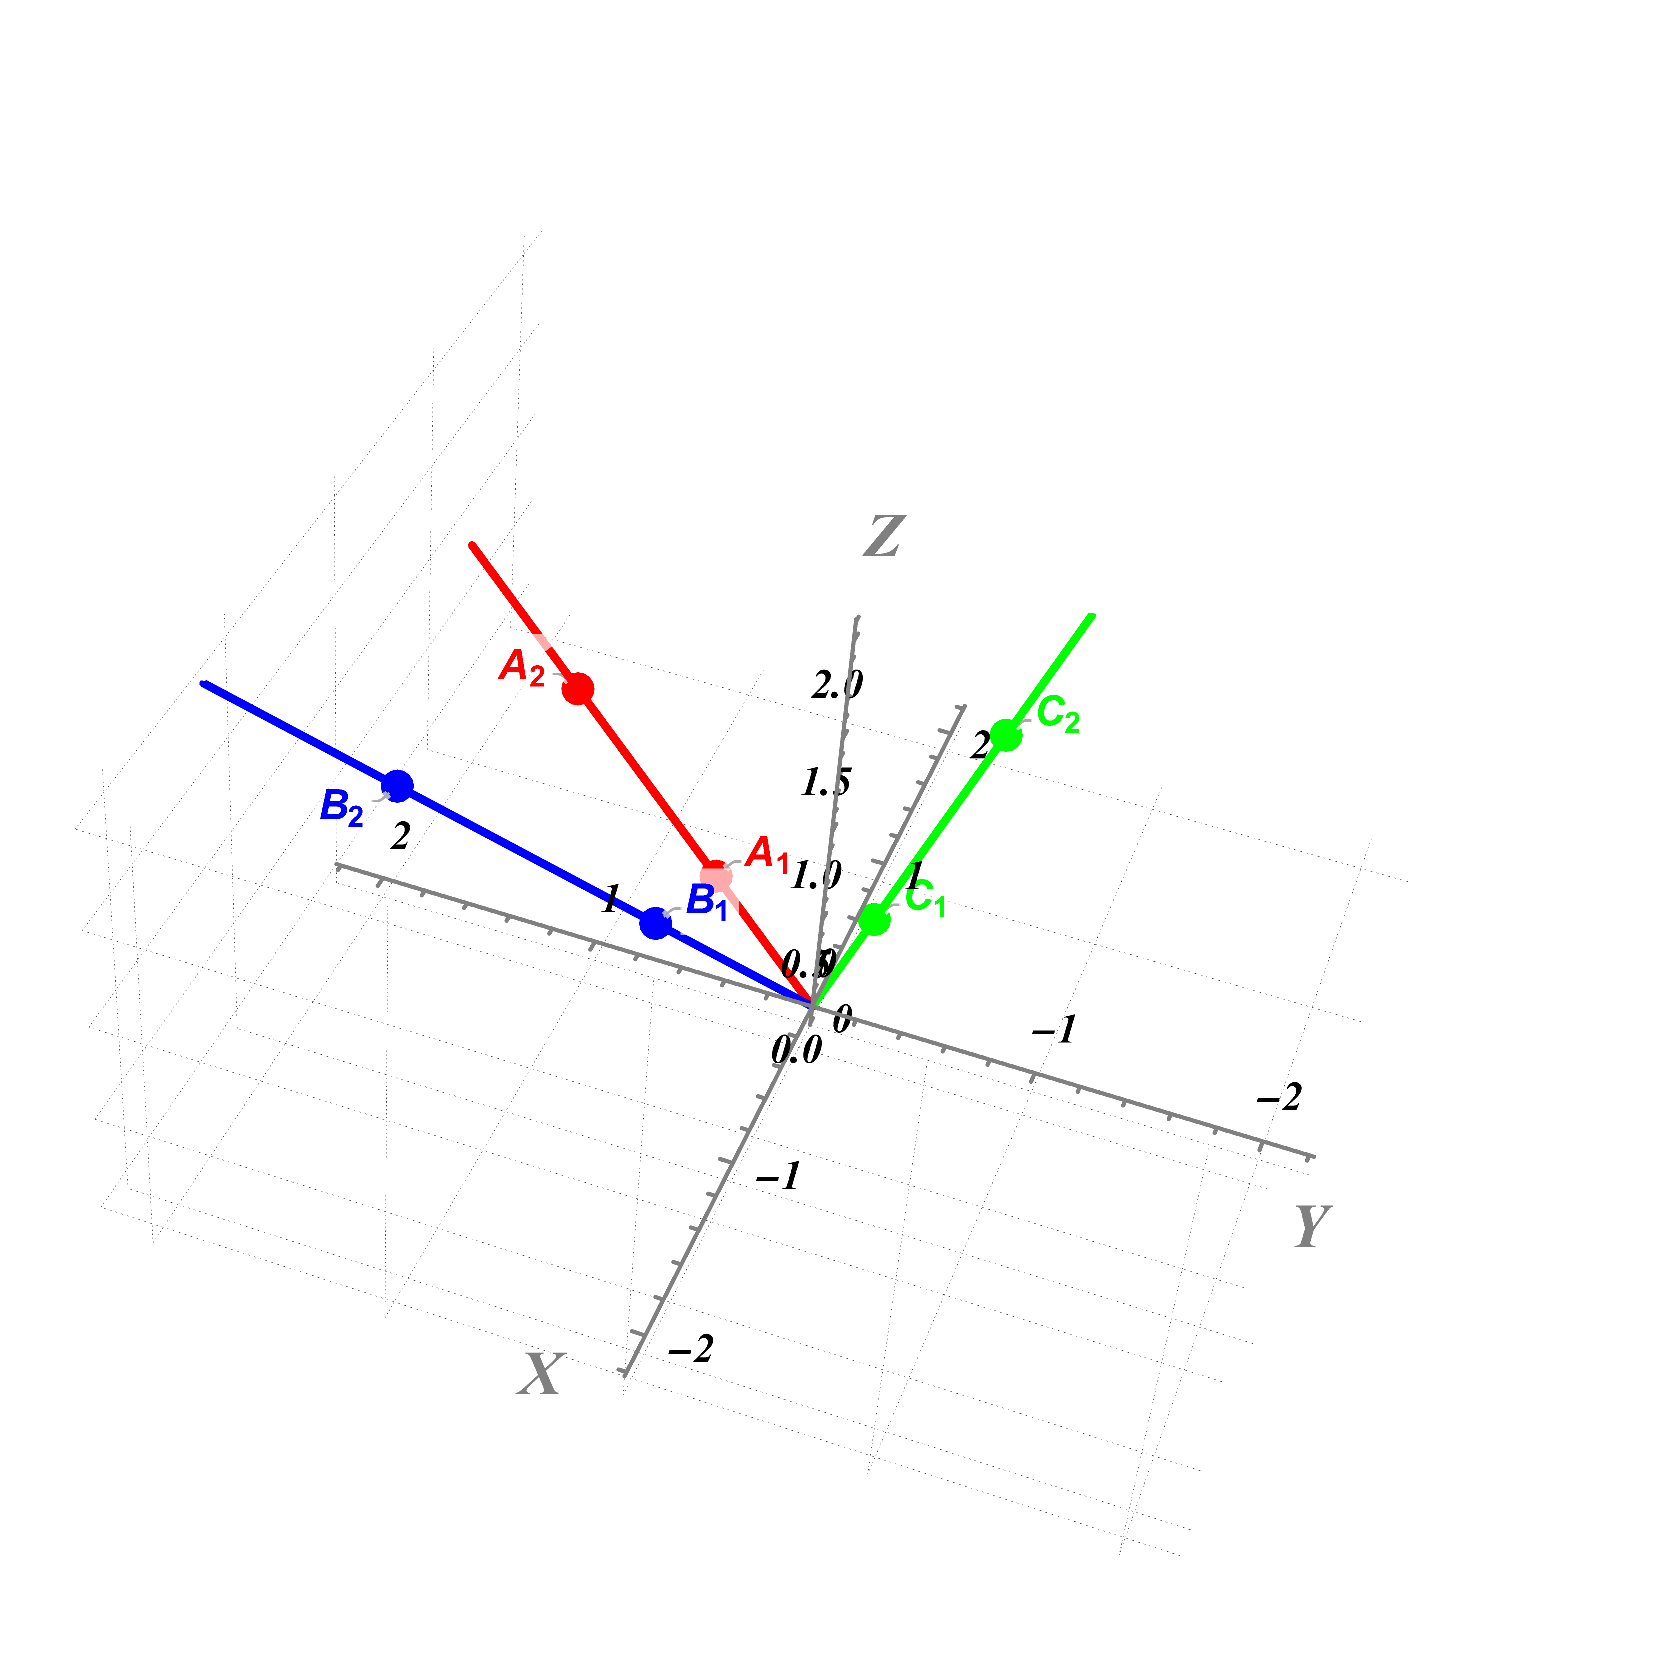
\includegraphics[trim={100 100 100 200}, width=0.45\linewidth, clip]{images/lecture_4/line_1_view_1.pdf} &
            \centering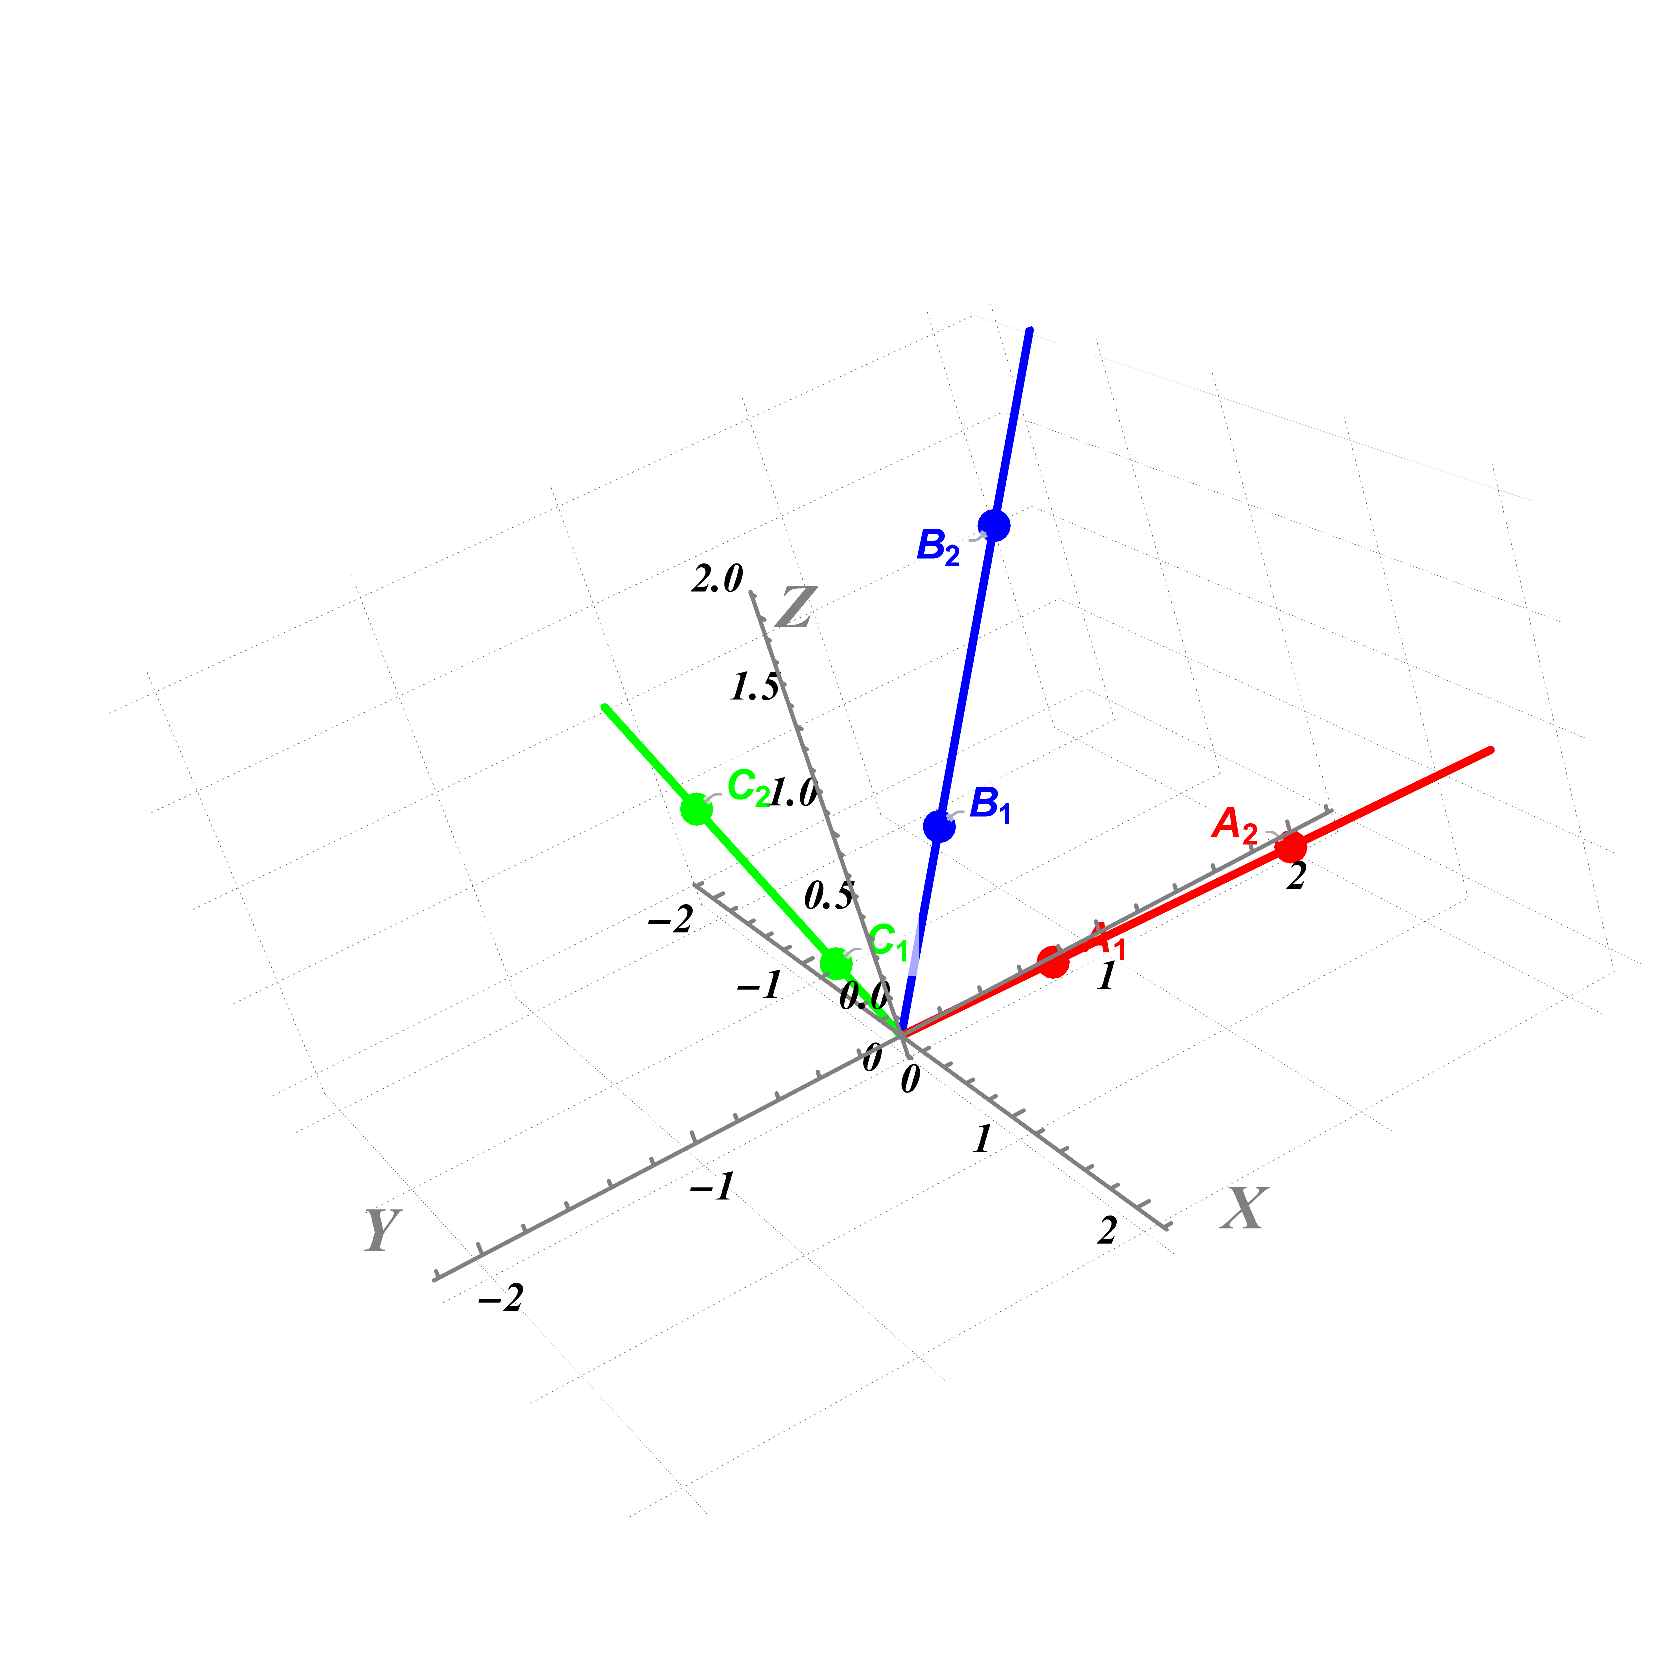
\includegraphics[trim={100 100 100 200}, width=0.45\linewidth, clip]{images/lecture_4/line_1_view_2.pdf}
        \end{tabular}
        \scriptsize{\textbf{Illustration:} Geometric interpretation of $\mathbb{P}^2(\mathbb{R})$, the same scene from different perspectives. The \textcolor{red}{\textbf{red}} line is represented by equation $(2t,3t,t)$, \textcolor{blue}{\textbf{blue}} line by $(-2t,3t,3t)$, and \textcolor{green!60!black}{\textbf{green}} line is represented by $(t,-2t,5t)$ for parameter $t \in \mathbb{R}$.}
    \end{center}

    Here, the figure demonstrates three equivalence classes, being a set of points on the \textcolor{red}{\textbf{red}}, \textcolor{blue}{\textbf{blue}}, and \textcolor{green!60!black}{\textbf{green}} lines (except for the origin). 
    
    The reason why geometrically the set of equivalence classes lie on the same line that passes through the origin is following: suppose we have a point $\vec{v}_0 = (x_0,y_0,z_0) \in \mathbb{R}^3$, represented as a vector. Then, the set of all points that are equivalent to $(x_0,y_0,z_0)$ is the set of all points $(\lambda x_0, \lambda y_0, \lambda z_0) = \lambda\vec{v}_0$ for $\lambda \in \mathbb{R}\setminus \{0\}$. So $\vec{v}_0$ is the representative of equivalence class $[\vec{v_0}] = \{\lambda\vec{v}_0: \lambda \in \mathbb{R},\lambda \neq 0\}$. Now notice, that this is a parametric equation of a line that passes through the origin and the point $\vec{v}_0$: notice that for $\lambda=0$ (if we assume that expression is also defined for zero $\lambda$) we have the origin $\vec{0}$, while for $\lambda=1$ we have the point $\vec{v}_0$. Then, any other values of $\lambda$ in-between $[0,1]$ or outside define the set of points lying on the same line.
\end{example}

Now, projective coordinates are not that useful unless we can come back to the affine space. This is done by defining the map $\phi: \mathbb{P}^2(\overline{\mathbb{K}}) \to \mathbb{A}^2(\overline{\mathbb{K}})$ as follows: $\phi: (X:Y:Z) \mapsto \left(X/Z, Y/Z\right)$. If, in turn, we want to go from the affine space to the projective space, we can define the map $\psi: \mathbb{A}^2(\overline{\mathbb{K}}) \to \mathbb{P}^2(\overline{\mathbb{K}})$ as follows: $\psi: (x,y) \mapsto (x:y:1)$. Geometrically, map $\phi$ means that we take a point $(X:Y:Z)$ and project it onto the plane $Z=1$.

\begin{example}
    Again, consider three lines from the previous example. Now, we additionally draw a plane $\pi: z=1$ in our 3-dimensional space (see Illustration below).

    \begin{center}
        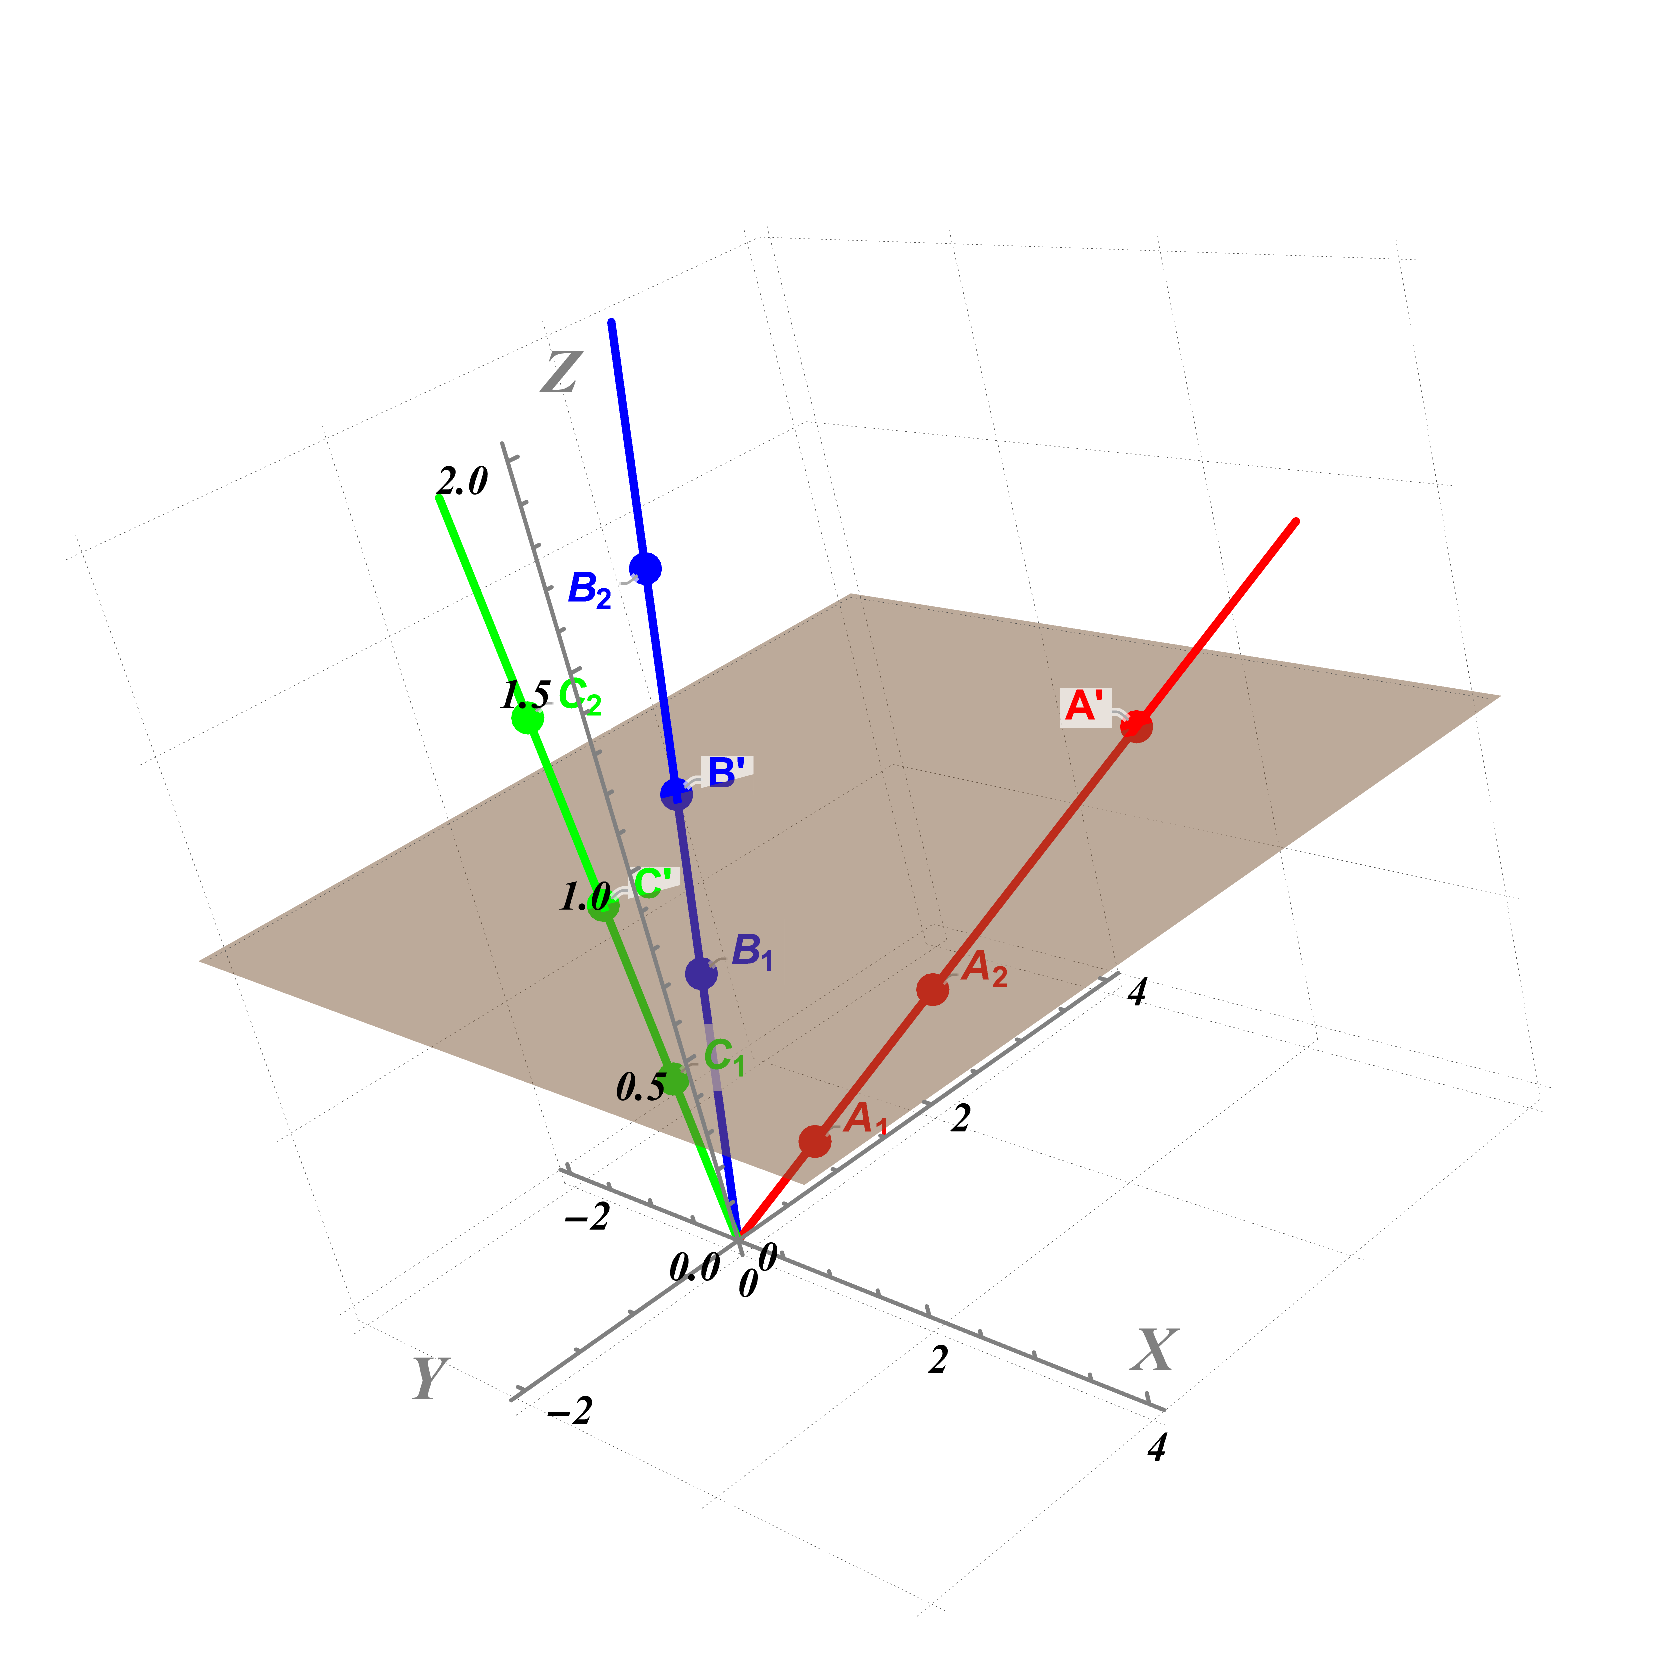
\includegraphics[trim={100 100 100 200}, width=0.45\linewidth, clip]{images/lecture_4/line_2.pdf}
        
        \scriptsize{\textbf{Illustration:} Geometric interpretation of converting projective form to the affine form.}
    \end{center}

    By using the map $(X:Y:Z) \mapsto (X/Z,Y/Z)$, all points on the line get mapped to the itersection of the line with the plane $\pi: z=1$. This way, for example, points on the \textcolor{red}{\textbf{red line}} $\ell_{\text{red}}$ get mapped to the point $A'=(2,3,1)$, corresponding to $(2,3)$ in affine coordinates. So, for example, point $(6,9,3) \in \ell_{\text{red}}$, lying on the same line, gets mapped to $(6/3,9/3) = (2,3)$.

    Similarly, all \textcolor{blue}{\textbf{blue line}} points get mapped to the point $B'=(-2/3,1,1)$, while all \textcolor{green!60!black}{\textbf{green line}} points get mapped to the point $C'=(0.2,-0.4,1)$\footnote{One can verify that based on the equations provided from the previous example}.
\end{example}

\subsubsection{Elliptic Curve Equation in Projective Form}

Now, quite an interesting question is following: how to represent (basically, rewrite) the ``affine'' elliptic curve equation\footnote{Further, we will use notation $E_{\mathbb{A}}$ to represent the elliptic curve equation in the affine form, and $E_{\mathbb{P}}$ to represent the elliptic curve in the projective form.}
\begin{equation}
    E_{\mathbb{A}}(\overline{\mathbb{F}}_p): y^2 = x^3 + ax + b, \; a,b \in \overline{\mathbb{F}}_p
\end{equation}
in the projective form? Since currently, we defined the curve as the 2D curve, but now we are working in 3D space! The answer is following: recall that if $(X:Y:Z) \in \mathbb{P}^2(\overline{\mathbb{F}}_p)$ lies on the curve, so does the point $(X/Z,Y/Z)$. The condition on the latter point to lie on $E_{\mathbb{A}}(\overline{\mathbb{F}}_p)$ is following:
\begin{equation}
    \left(\frac{Y}{Z}\right)^2 = \left(\frac{X}{Z}\right)^3 + a\cdot \frac{X}{Z} + b
\end{equation}

But now multiply both sides by $Z^3$ to get rid of the fractions:
\begin{equation}
    E_{\mathbb{P}}(\overline{\mathbb{F}}_p): Y^2Z = X^3 + aXZ^2 + bZ^3
\end{equation}

This is an equation of the elliptic curve in \textbf{projective form}. 

Now, one of the motivations to work with the projective form was to unify affine points $E_{\mathbb{A}}/\overline{\mathbb{F}}_p$ and the point at infinity $\mathcal{O}$, which acted as an identity element in the group $E_{\mathbb{A}}(\overline{\mathbb{F}}_p)$. So how do we encode the point at infinity in the projective form?

Well, notice the following observation: all points $(0:\lambda:0)$ always lie on the curve $E_{\mathbb{P}}(\overline{\mathbb{F}}_p)$. Moreover, the map from the projective form to the affine form is ill-defined for such points, since we would need to divide by zero. So, we can naturally make the points $(0:\lambda:0)$ to be the set of points at infinity. This way, we can define the point at infinity as $\mathcal{O} = (0:1:0)$.

Finally, let us summarize what we have observed so far.

\begin{definition}
    The \textbf{homogenous projective form of the elliptic curve} $E_{\mathbb{P}}(\overline{\mathbb{F}}_p)$ is defined as the set of all points $(X:Y:Z) \in \mathbb{P}^2(\overline{\mathbb{F}}_p)$ in the projective space that satisfy the equation
    \begin{equation}
        E_{\mathbb{P}}(\overline{\mathbb{F}}_p): Y^2Z = X^3 + aXZ^2 + bZ^3, \;\; a,b \in \overline{\mathbb{F}}_p,
    \end{equation}
    where the point at infinity is encoded as $\mathcal{O} = (0:1:0)$.
\end{definition}

\begin{example}
    Consider the BN254 curve $y^2 = x^3 + 3$ over reals $\mathbb{R}$. Its projective form is given by the equation $Y^2Z = X^3 + 3Z^3$, which gives a surface, depicted below.
    \begin{center}
        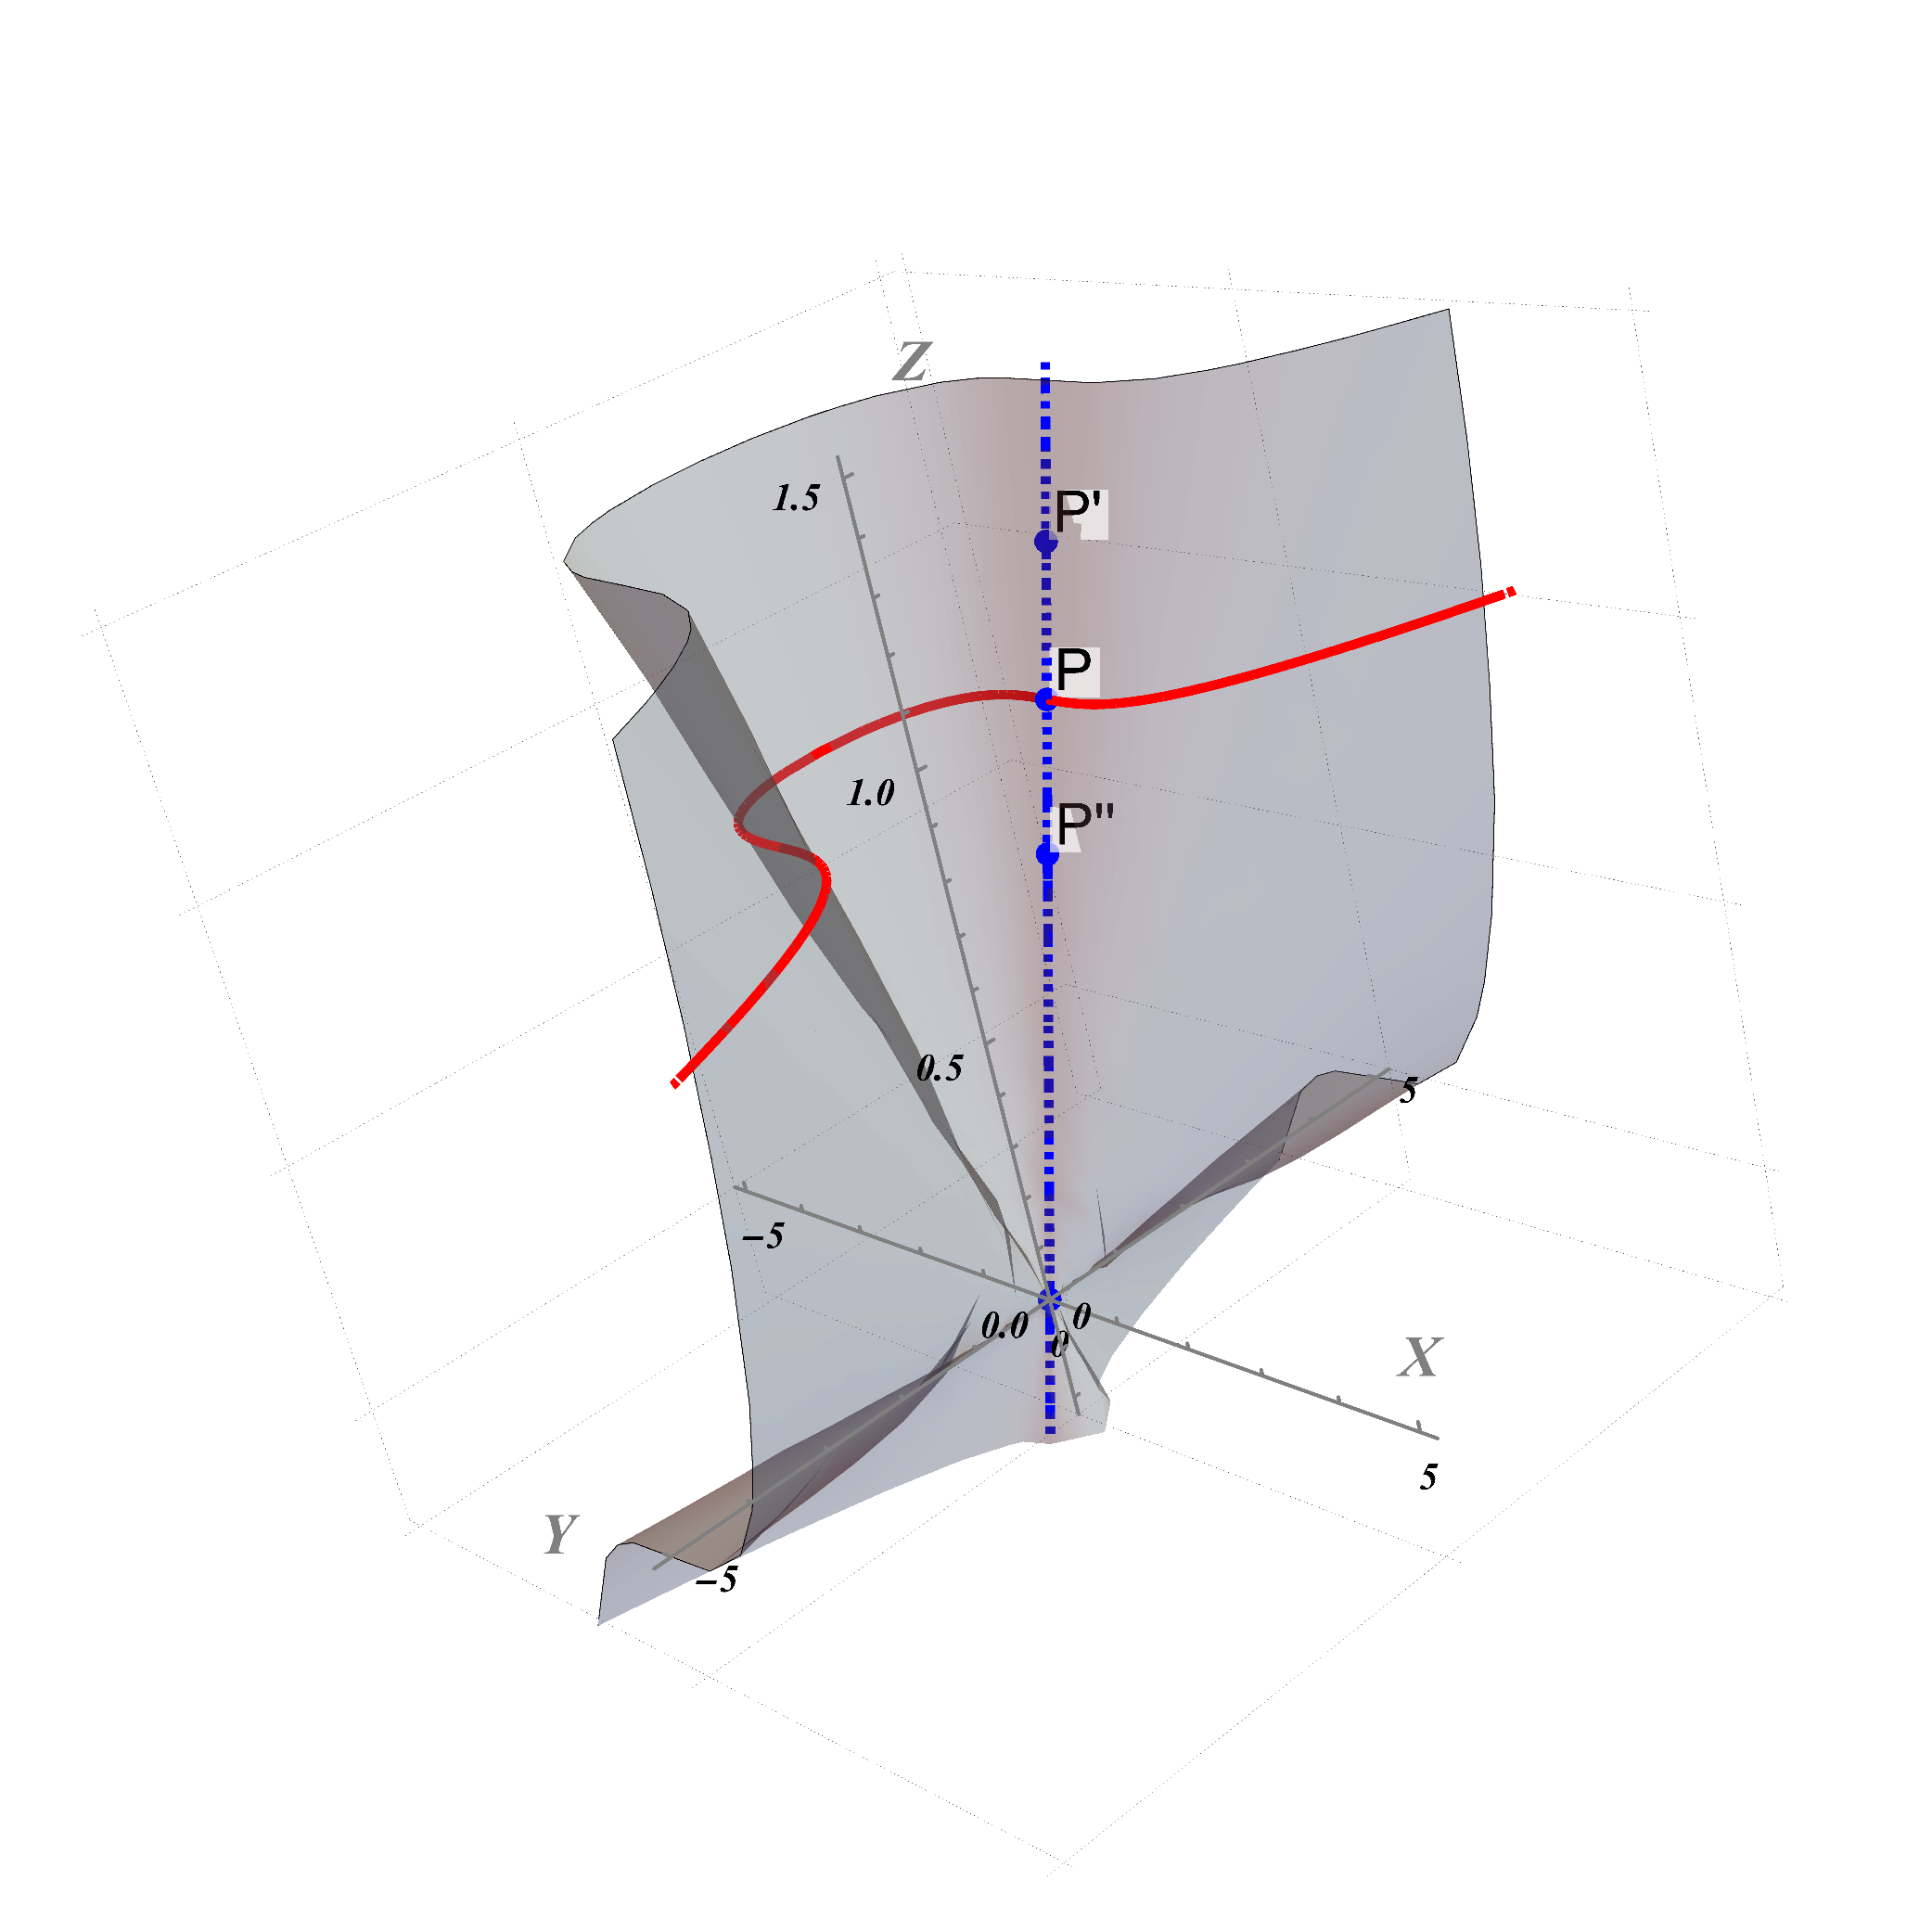
\includegraphics[trim={275 100 225 100}, width=0.35\linewidth, clip]{images/lecture_4/projective_ec.pdf}
        
        \scriptsize{\textbf{Illustration:} BN254 Curve Elliptic Curve in Projective Form over $\mathbb{R}$. In \textcolor{black!80}{\textbf{gray}} is the surface, while \textcolor{red}{\textbf{red}} points are the points on the affine curve (lying on the plane $\pi: z=1$).}
    \end{center}

    Points $P'\approx (0:2.165:1.25)$ and $P'' \approx (0:1.3:0.75)$ in projective form both lie on the curve and get mapped to the same point $P \approx (0,1.732)$ in affine coordinates.
\end{example}

\subsubsection{General Projective Coordinates}
Hold on, but why did we use the term \textit{homogenous}? The reason why is because we defined equivalence as follows: $(X:Y:Z) \sim (\lambda X: \lambda Y: \lambda Z)$ for some $\lambda \in \overline{\mathbb{K}}$, called \textbf{homogenous coordinates}. However, this is not the only way to define equivalence. Consider a more general form of equivalence relation:
\begin{equation}
    (X:Y:Z) \sim (X':Y':Z') \;\; \text{iff} \;\; \exists \lambda \in \overline{\mathbb{K}}: (X,Y,Z) = (\lambda^n X', \lambda^m Y', \lambda Z')
\end{equation}

In this case, to come back to the affine form, we need to use the map $\phi: (X:Y:Z) \mapsto (X/Z^n, Y/Z^m)$. 
\begin{example}
    The case $n=2,m=3$ is called the \textbf{Jacobian Projective Coordinates}. An Elliptic Curve equation might be then rewritten as: 
    \begin{equation}
        Y^2 = X^3 + aXZ^4 + bZ^6
    \end{equation}
    The reason why we might want to use such coordinates is that they can be more efficient in some operations, such as point addition. However, we will not delve into this topic much further.
\end{example}

\begin{example}
    Consider the BN254 curve $y^2 = x^3 + 3$ over reals $\mathbb{R}$, again. Its \textit{Jacobian projective form} is given by the equation $Y^2 = X^3 + 3Z^6$, which gives a surface, depicted below.
    \begin{center}
        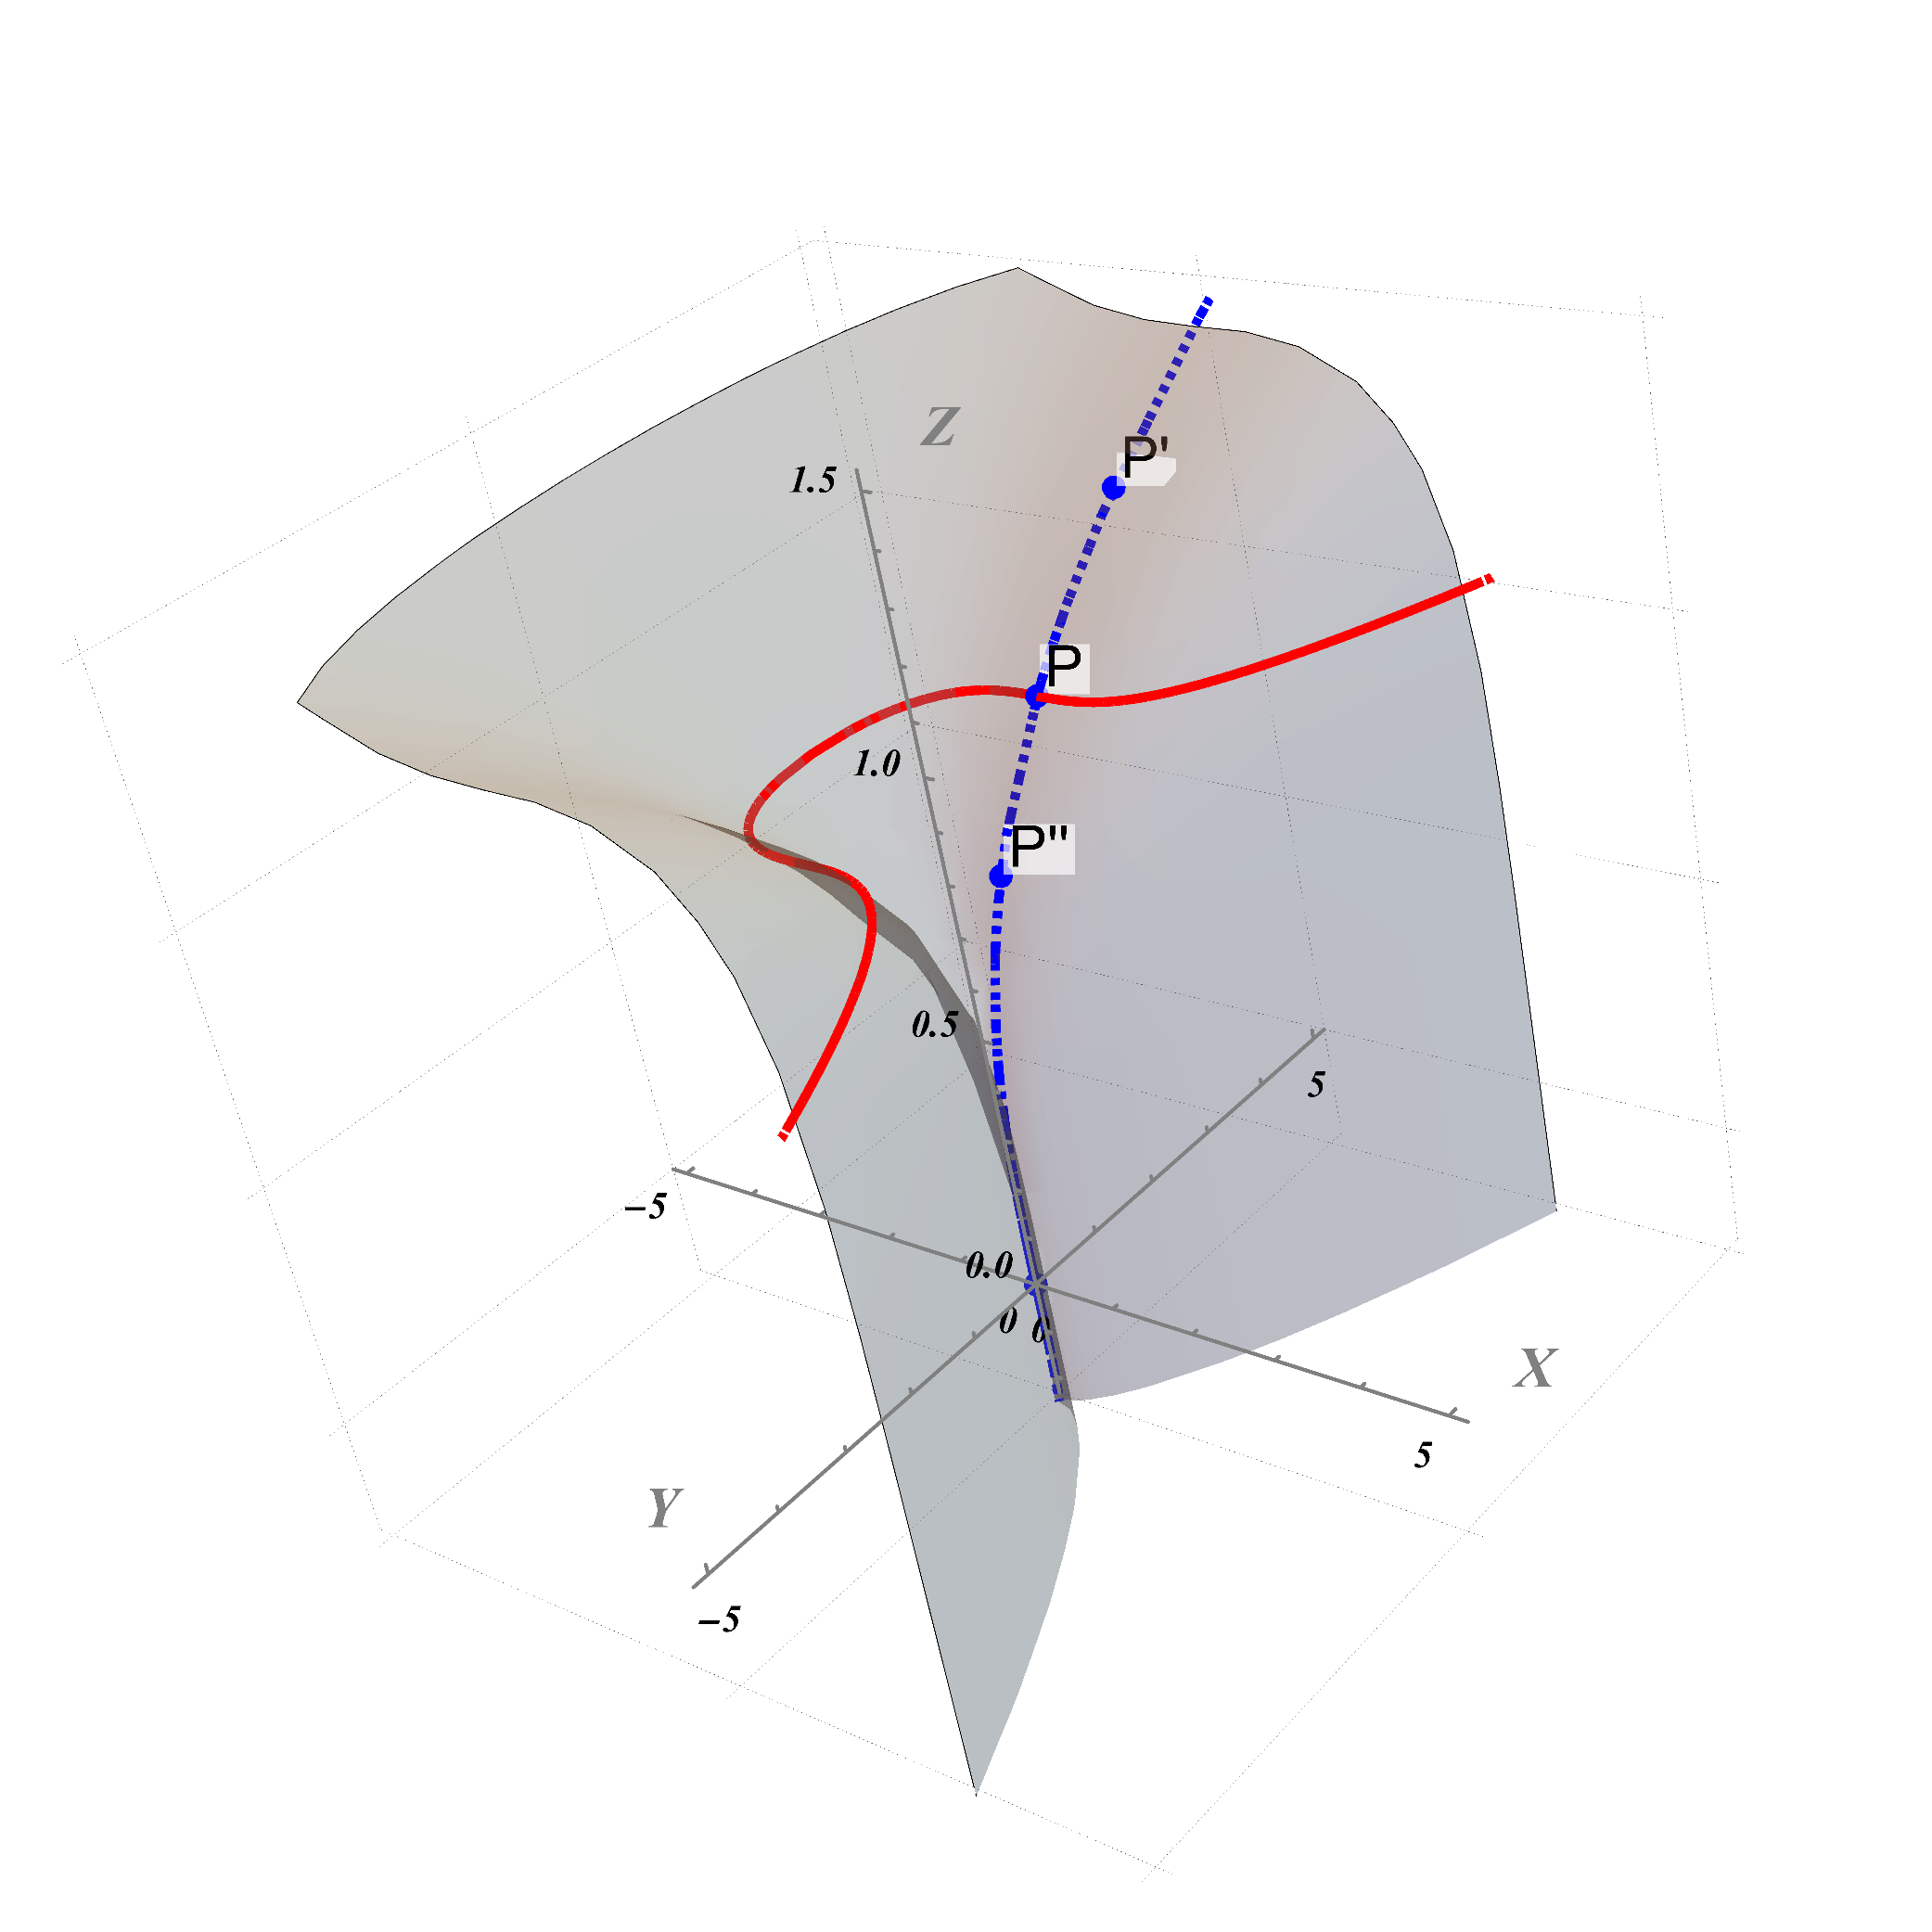
\includegraphics[trim={275 140 225 100}, width=0.35\linewidth, clip]{images/lecture_4/projective_ec_jacobian.pdf}
        
        \scriptsize{\textbf{Illustration:} BN254 Curve Elliptic Curve in Jacobian Projective Form over $\mathbb{R}$. In \textcolor{black!80}{\textbf{gray}} is the surface, while \textcolor{red}{\textbf{red}} points are the points on the affine curve (lying on the plane $\pi: z=1$).}
    \end{center}

    Notice that now, under the map $(X:Y:Z) \mapsto (X/Z^2,Y/Z^3)$, points in the same equivalence class (in $\mathbb{R}^3$) do not lie on the same line, but rather on the same \textit{curve}. Namely, equivalence class has a form $[(x_0,y_0,z_0)] = \{t^2x_0,t^3y_0,tz_0: t \in \mathbb{R} \setminus \{0\}\}$.
\end{example}

\subsubsection{Fast Addition}

Let us come back to the affine case and assume that the underlying field is the prime field $\mathbb{F}_p$. Recall that for adding two points $P=(x_P,y_P)$ and $Q=(x_Q,y_Q)$ to get $R=(x_R,y_R) \gets P \oplus Q$ one used the following formulas (there is no need to understand the derivation fully, just take it as a fact):
\begin{equation}
    x_R \gets \left(\frac{y_Q-y_P}{x_Q-x_P}\right)^2 - x_P - x_Q, \;\;\; y_R \gets \left(\frac{y_Q-y_P}{x_Q-x_P}\right)(x_P-x_R) - y_P
\end{equation}

Denote by $\textcolor{blue}{\mathsf{M}}$ the cost of multiplication, by $\textcolor{green!60!black}{\mathsf{S}}$ the cost of squaring, and by $\textcolor{red}{\mathsf{I}}$ the cost of inverse operation in $\mathbb{F}_p$. Note that we do not count addition/inverse costs as they are significantly lower than operations listed. Then, the cost of additing two points using above formula is $2\textcolor{blue}{\mathsf{M}} + 1\textcolor{green!60!black}{\mathsf{S}} + 1\textcolor{red}{\mathsf{I}}$. Indeed, our computation can proceed as follows:
\begin{enumerate}
    \item Calculate $t_1 \gets (x_Q-x_P)^{-1}$, costing $1\textcolor{red}{\mathsf{I}}$.
    \item Calculate $\lambda \gets (y_Q-y_P)t_1$, costing $1\textcolor{blue}{\mathsf{M}}$.
    \item Calculate $t_2 \gets \lambda^2$, costing $1\textcolor{green!60!black}{\mathsf{S}}$.
    \item Calculate $x_R \gets t_2 - x_P - x_Q$, costing almost nothing.
    \item Calculate $y_R \gets \lambda (x_P-x_R) - y_P$, costing $1\textcolor{blue}{\mathsf{M}}$.
\end{enumerate}

Well, there are just 4 operations in total, so what can go wrong? The problem is that we need to calculate the inverse of $(x_Q-x_P)$, which is a very, very costly operation. In fact, typically $1\textcolor{red}{\mathsf{I}} \gg 20\textcolor{blue}{\mathsf{M}}$ or even worse, the ratio might reach $80$ in certain cases.

Now imagine we want to add 4 points, say $P_1 \oplus P_2 \oplus P_3 \oplus P_4$: this costs $6\textcolor{blue}{\mathsf{M}} + 3\textcolor{green!60!black}{\mathsf{S}} + 3\textcolor{red}{\mathsf{I}}$. Now we have 3 inverses, which is a lot. Finally, if we are to add much larger number of points (for example, when finding the scalar product), this gets even worse. 

Projective coordinates is a way to solve this problem. The idea is to represent points in the projective form $(X:Y:Z)$, so when adding two numbers in projective form, you still get a point in a form $(X:Y:Z)$. Then, after conducting a series of additions, you can convert the point back to the affine form. 

But why adding two points, say, $(X_P:Y_P:Z_P)$ and $(X_Q:Y_Q:Z_Q)$, in the projective form is more efficient? We will not derive the formulas, but trust us that they have the following form:
\begin{equation}
    \begin{aligned}
        X_R = (X_PZ_Q - X_QZ_P)(Z_PZ_Q(Y_PZ_Q-Y_QZ_P)^2 - (X_PZ_Q-X_QZ_P)^2(X_PZ_Q+X_QZ_P)); \\
        Y_R = Z_PZ_Q(X_QY_P - X_PY_Q)(X_PZ_Q-X_QZ_P)^2 - (Y_PZ_Q-Y_QZ_P)((Y_PZ_Q-Y_QZ_P)^2Z_PZ_Q\\-(X_PZ_Q+X_QZ_P)(X_PZ_Q-X_QZ_P)^2); \\
        Z_R = Z_PZ_Q(X_PZ_Q - X_QZ_P)^3.
    \end{aligned}
\end{equation}

Do not be afraid, you do not need to understand how this formula is derived. But notice that despite the very scary look, there is no inversions involved! Moreover, this formula can be calculated in only $12\textcolor{blue}{\mathsf{M}}+2\textcolor{green!60!black}{\mathsf{S}}$! So all in all, this is much more effective than $2\textcolor{blue}{\mathsf{M}} + 1\textcolor{green!60!black}{\mathsf{S}} + 1\textcolor{red}{\mathsf{I}}$.

The only inversion which is unavoidable in the projective form is the inversion of $Z$ since after all additions (and doublings) have been made, we need to use map $(X:Y:Z) \mapsto (X/Z,Y/Z)$ to return back to the affine form. However, this inversion is done only once at the end of the computation, so it is not that costly.

\begin{proposition}
    To conclude, typically, when working with elliptic curves, one uses the following strategy:
    \begin{enumerate}
        \item Convert affine points to projective form using the map $(x,y) \mapsto (x,y,1)$.
        \item Perform all operations in the projective form, which do not involve inversions.
        \item Convert the result back to the affine form using the map $(X:Y:Z) \mapsto (X/Z,Y/Z)$.
    \end{enumerate}

    This is illustrated in the Figure below.
    \begin{center}
        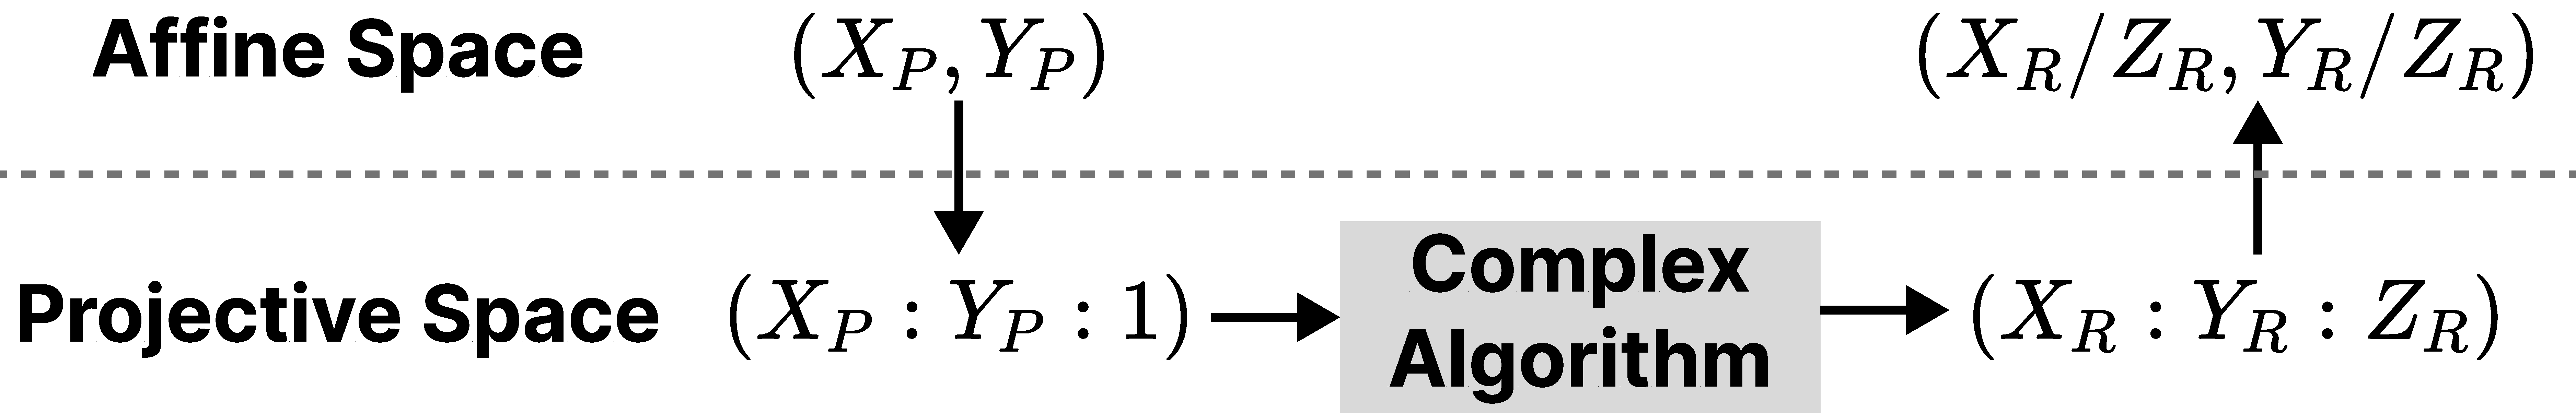
\includegraphics[width=0.8\linewidth]{images/lecture_4/strategy.pdf}
        
        \scriptsize{\textbf{Illustration:} General strategy when performing operations over Elliptic Curves.}
    \end{center}
\end{proposition}

\subsubsection{Scalar Multiplication Basic Implementation}

Now, the question is: how do we implement the scalar multiplication $[k]P$ for the given scalar $k \in \mathbb{Z}_r$ and point $P \in E(\overline{\mathbb{F}}_q)$? 

First idea: let us simply add $P$ to itself $k$ times. Well, the complexity would be $O(k)$ in this case, which is even harder than solving the discrete logarithm problem (recall that the discrete logarithm problem has a complexity of $O(\sqrt{k})$). Yikes.

So there should be a better way. In this section we will limit ourselves to the double-and-add method, but the curious reader can look up the NAF (Non-Adjacent Form) method, windowed methods, GLV scalar decomposition and many other methods, which we are not going to cover in this course.

The idea of the double-and-add method is following: we represent the $N$-bit scalar $k$ in binary form, say $k = (k_{N-1},k_{N-2},\dots,k_0)_2$, then we calculate $P, [2]P, [4]P, [8]P, \dots, [2^{N-1}]P$ (which is simply applying the doubling multple times) and then add the corresponding points (corresponding to positions where $k_i=1$) to get the result. Formally, we specify the \Cref{alg:double_and_add}.

\begin{algorithm}
    \caption{Double-and-add method for scalar multiplication}\label{alg:double_and_add}
    \Input{$P \in E(\mathbb{F}_q)$ and $k \in \mathbb{Z}_{r}$}
    \Output{Result of scalar multiplication $[k]P \in E(\mathbb{F}_q)$}
    
    Decompose $k$ to the binary form: $(k_0,k_1,\dots,k_{N-1})$
    
    $R \gets \mathcal{O}$
    
    $T \gets P$
    
    \For{$i \in \{0,\dots,N-1\}$}{
        \If{$k_i = 1$}{
            $R \gets R \oplus T$
        }
    
        $T \gets [2]T$
    }
    
    \Return{Point $R$}
\end{algorithm}    

Good news: now we have a complexity of $O(N)=O(\log k)$, which is way much better that a linear one. In fact, many more optimized methods have the same assymptotic complexity (meaning, a logarithmic one), so it turns out that 
we cannot do much better than that. However, the main advantages of other, more optimized methods is that we can avoid making too many additions (here, in the worst case, we have to make $N$ additions), which is a costly operation (and more expensive than doubling).

Moreover, here we can use projective coordinates to make the addition and doubling operation more efficient! After all, typically the number of operations is even more than $300$, so making $300$ inversions in affine form is not an option.

\subsection{Elliptic Curve Pairing}

Pairing is the core object used in threshold signatures, zk-SNARKs constructions, and other cryptographic applications. 

Consider the \textit{Decisional Diffie-Hellman problem} which we considered in \Cref{section:math-crypto-2} (based on $g^{\alpha},g^{\beta}$ and $g^{\gamma}$, decide whether $\gamma = \alpha\beta$). Turns out that for curves where the so-called \textit{embedding degree}\footnote{We will mention what that is is later, but still this term is quite hard to define.} is small enough, this problem is easy to solve. This might sound 
like a quite bad thing, but it turns out that although some information about the discrete logarithm is leaked, it is not enough to break the security of the system (basically, solve the \textit{Computational Diffie-Hellman problem}). 
Pairings is the exact object that allows us to solve the Decisional Diffie-Hellman problem.

However, a more interesting use-case which we are going to use in SNARKs is that pairings allows us to check \textbf{quadratic conditions} on scalars using their corresponding elliptic curve representation. For example, just given $u=g^{\alpha},v=g^{\beta}$ we can check whether $\alpha\beta+5=0$ (which is impossible to check without having a pairing). 

So what is pairing?

\subsubsection{Definition}

\begin{definition}
    \textbf{Pairing} is a bilinear, non-degenerate, efficiently computable map $e: \textcolor{red}{\mathbb{G}_1} \times \textcolor{blue}{\mathbb{G}_2} \to \textcolor{ForestGreen}{\mathbb{G}_T}$, where $\textcolor{red}{\mathbb{G}_1},\textcolor{blue}{\mathbb{G}_2}$ are two groups (typically, elliptic curve groups) and $\textcolor{ForestGreen}{\mathbb{G}_T}$ is a target group (typically, a set of scalars). Let us decipher the definition:
    \begin{itemize}
        \item \textbf{Bilinearity} means essentially the following:
        \begin{equation*}
            e([a]\textcolor{red}{P},[b]\textcolor{blue}{Q}) = e([ab]\textcolor{red}{P},\textcolor{blue}{Q}) = e(\textcolor{red}{P},[ab]\textcolor{blue}{Q}) = e(\textcolor{red}{P},\textcolor{blue}{Q})^{ab}.        
        \end{equation*}
        \item \textbf{Non-degeneracy} means that $e(G_1,G_2) \neq 1$ (where $G_1,G_2$ are generators of $\textcolor{red}{\mathbb{G}_1},\textcolor{blue}{\mathbb{G}_2}$, respectively). This property basically says that the pairing is not trivial.
        \item \textbf{Efficient computability} means that the pairing can be computed in a reasonable time.
    \end{itemize}

    The definition is illustrated in \Cref{fig:ecpairing}.
\end{definition}

\begin{figure}[H]
    \centering
    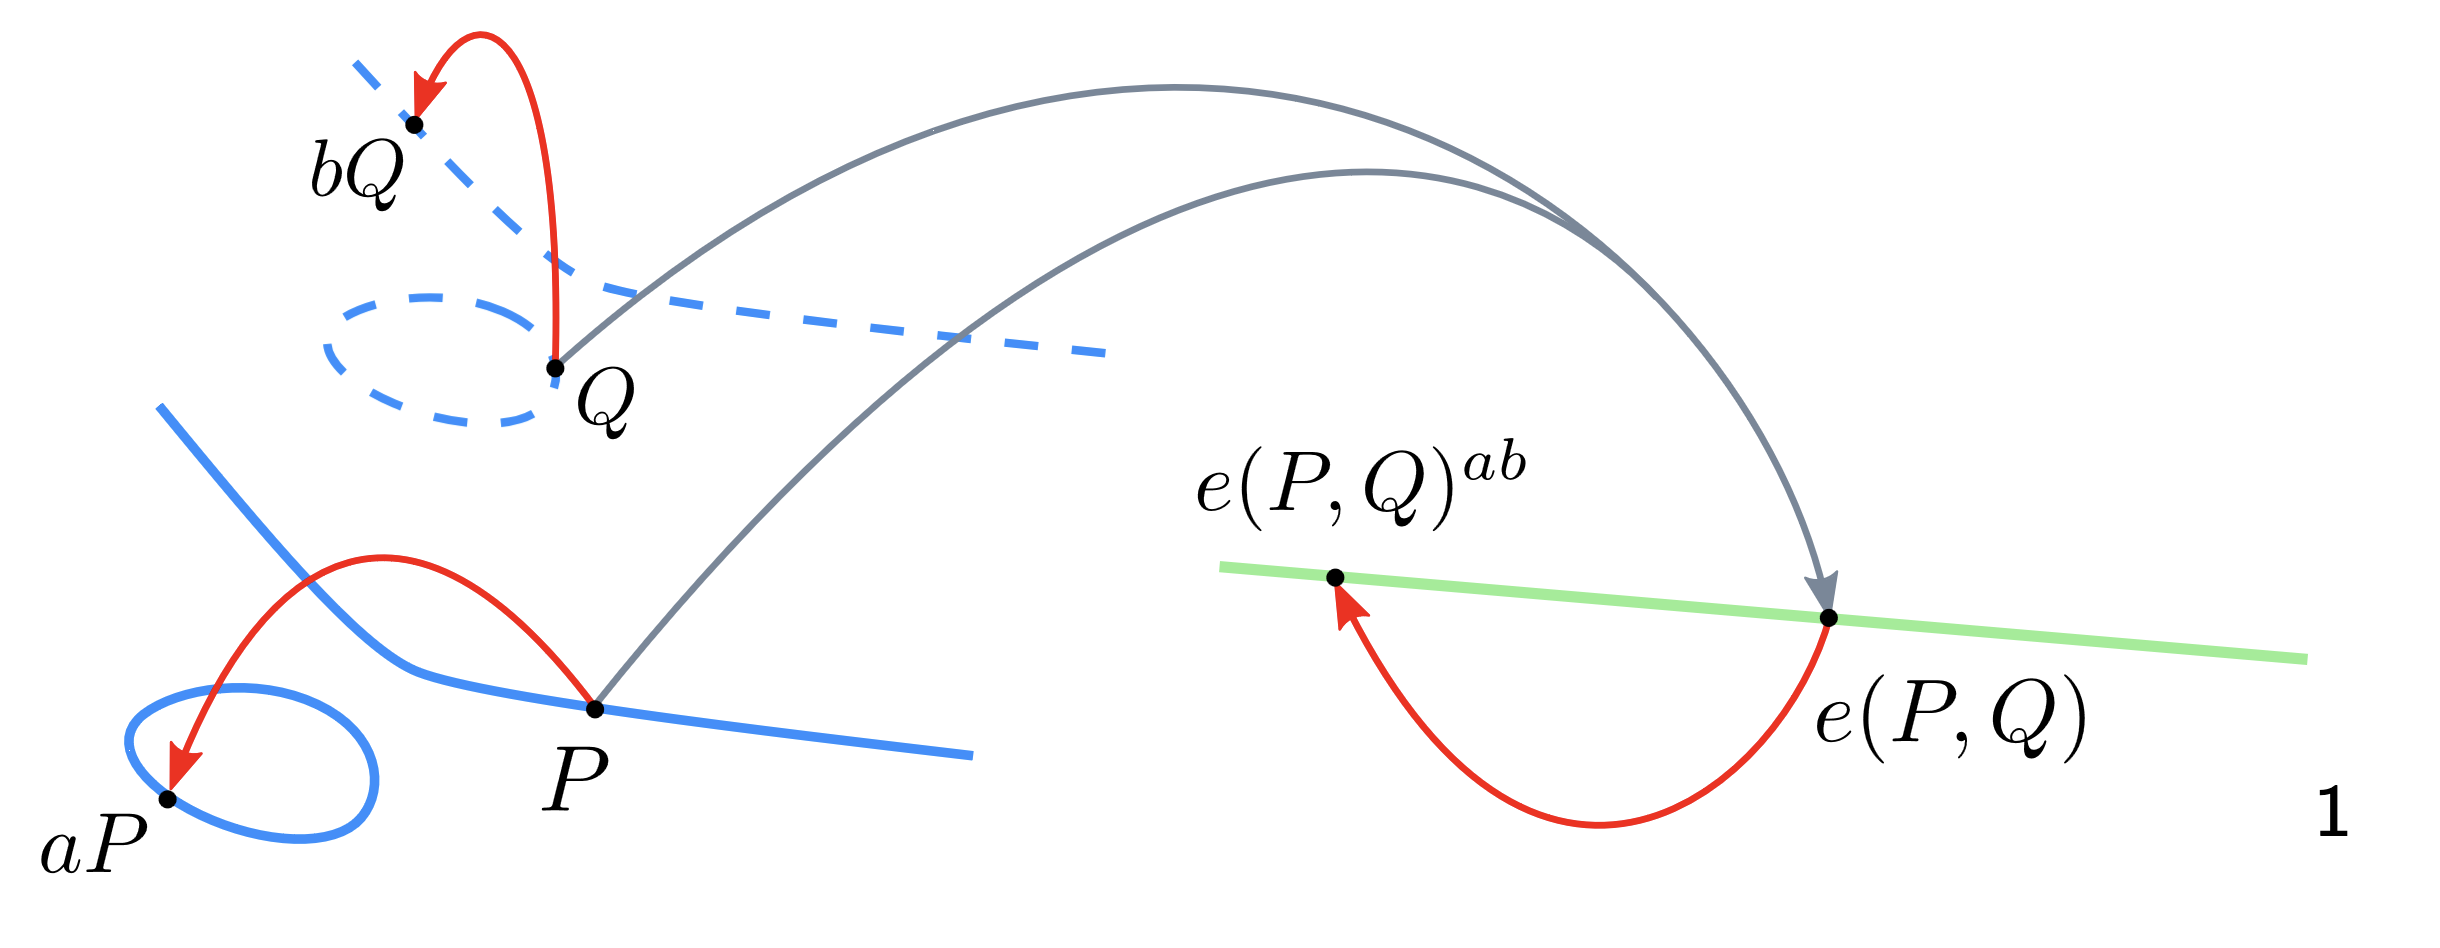
\includegraphics[width=0.75\textwidth]{images/lecture_4/pairing.png}
    \caption{Pairing illustration. It does not matter what we do first: (a) compute $[a]P$ and $[b]Q$ and then compute $e([a]P,[b]Q)$ or (b) first calculate $e(P,Q)$ and then transform it to $e(P,Q)^{ab}$. \scriptsize{Figure taken from ``Pairings in R1CS'' talk by Youssef El Housni}}
    \label{fig:ecpairing}
\end{figure}

\begin{example}
    Suppose $\mathbb{G}_1=\mathbb{G}_2=\mathbb{G}_T=\mathbb{Z}_r$ are scalars. Then, the map $e: \mathbb{G}_1 \times \mathbb{G}_2 \to \mathbb{G}_T$, defined as:
    \begin{equation}
        e(x,y)= 2^{xy}
    \end{equation}
    is pairing. Indeed, it is bilinear. For example, $e(ax,by) = 2^{abxy} = (2^{xy})^{ab} = e(x,y)^{ab}$ or $e(ax,by)=2^{abxy}=2^{(x)(aby)}=e(x,aby)$. Moreover, it is non-degenerate, since $e(1,1)=2 \neq 1$. And finally, it is obviously efficiently computable.

    However, this is a quite trivial example since working over integers is typically not secure. For example, the discrete logarithm over $\mathbb{Z}_r$ can be solved in subexponential time. For that reason, we want to build pairings over elliptic curves.
\end{example}

\begin{example}
    \textbf{Pairing for BN254.} For BN254 (with equation $y^2=x^3+3$), the pairing function $e: \mathbb{G}_1 \times \mathbb{G}_2 \to \mathbb{G}_T$ is defined over the following groups:
    \begin{itemize}
        \item $\textcolor{red}{\mathbb{G}_1}$ --- points on the regular curve $E(\mathbb{F}_p)$.
        \item $\textcolor{blue}{\mathbb{G}_2}$ --- $r$-torsion points on the twisted curve $E'(\mathbb{F}_{p^2})$ over the field extension $\mathbb{F}_{p^2}$ (with equation $y^2 = x^3+\frac{3}{\xi}$ for $\xi=9+u \in \mathbb{F}_{p^2}$).
        \item $\textcolor{ForestGreen}{\mathbb{G}_T}$ --- $r$th roots of unity $\Omega_r \subset \mathbb{F}_{p^{12}}^{\times}$.
    \end{itemize}

    Well, this one is quite intense and even understanding the input and output parameters is quite hard. So let us decipher some components:
    \begin{itemize}
        \item \textbf{$r$-torsion subgroup on the curve $E(\mathbb{F}_{p^m})$} is simply a set of points, which multiplied by $r$ give the point at infinity (that is, $[r]P=\mathcal{O}$). Formally, $E(\mathbb{F}_{p^m})[r] = \{P \in E(\mathbb{F}_{p^m}): [r]P = \mathcal{O}\}$. Of course, for the curve $E(\mathbb{F}_p)$, the $r$-torsion subgroup is simply the whole curve, but that is generally not the case for the twisted curve over the extension field.
        \item \textbf{$r$th roots of unity} is a set of elements $\Omega_r = \{z \in \mathbb{F}_{p^{12}}^{\times}: z^r=1\}$. This is a group under multiplication, and it has exactly $r$ elements.
    \end{itemize}
\end{example}

\begin{remark}
    One might a reasonable question: where does this $12$ come from? The answer is following: the so-called \textbf{embedding degree} of BN254 curve is $k=12$. This number is the key to understanding why we are working over such large extensions when calculating the pairing. The formal description is quite hard, but the intuition is following: the embedding degree is the smallest number $k$ such that all the $r$th roots of unity lie inside the extended field $\mathbb{F}_{p^k}$. If $k$ was smaller, the output of pairing would contain less that $r$ points and some points would be missing, which would make the pairing more trivial. For that reason, we need to have $\Omega_r \subset \mathbb{F}_{p^k}$.
\end{remark}

\begin{definition}
    The following conditions are equivalent \textbf{definitions} of an embedding degree of an elliptic curve $E(\overline{\mathbb{F}}_p)$:
    \begin{itemize}
        \item $k$ is the smallest positive integer such that $r \mid (p^k-1)$.
        \item $k$ is the smallest positive integer such that $\mathbb{F}_{p^k}$ contains all of the $r$-th roots of unity in $\overline{\mathbb{F}}_p$, that is $\Omega_r \subset \mathbb{F}_{p^k}$.
        \item $k$ is the smallest positive integer such that $E(\overline{\mathbb{F}}_p)[r] \subset E(\mathbb{F}_{p^k})$
    \end{itemize}
\end{definition}

Pretty obvious observation: lower embedding degree is better, since it allows us to work over smaller fields. But usually, this embedding degree is quite large and we need to craft elliptic curves specifically to have a small embedding degree. For example, a pretty famous curve \texttt{secp256k1} has an embedding degree
\begin{equation*}
    k = \mathsf{0x2aaaaaaaaaaaaaaaaaaaaaaaaaaaaaaa74727a26728c1ab49ff8651778090ae0},
\end{equation*}
which is 254-bit long. For that reason, it is natural to define the term \textit{pairing-friendly elliptic curve}.
\begin{definition}
    An elliptic curve is called \textbf{pairing-friendly} if it has a relatively small embedding degree $k$ (typically, $k \leq 16$).
\end{definition}

\begin{remark}
    One might ask why usually, when dealing with pairings, we do not get to work with field extensions that much (most likely, if you were to write \texttt{groth16} from scratch using some mathematical libraries, you will not need to work with $\mathbb{F}_{p^{12}}$ arithmetic specifically). The reason is that typically, libraries implement the following abstraction: given a set of points $\{(P_i,Q_i)\}_{i=1}^n \subset \mathbb{G}_1^n \times \mathbb{G}_2^n$, the function checks whether
    \begin{equation}
        \prod_{i=1}^n e(P_i,Q_i) = 1
    \end{equation}
    Note that in this case, we do not need to work with $\mathbb{F}_{p^{12}}$ arithmetic, but rather checking the equality in the target group $\mathbb{G}_T$. 

    \textbf{Interesting fact:} this condition is specified in the \texttt{ecpairing} precompile standard used in Ethereum.
\end{remark}

\subsubsection{Case Study: BLS Signature}

One of the most elegant applications of pairings is the BLS Signature scheme. Compared to ECDSA or other signature schemes, BLS can be formulated in three lines.

Suppose we have pairing $e: \mathbb{G}_1 \times \mathbb{G}_2 \to \mathbb{G}_T$ (with generators $G_1,G_2$, respectively), and a hash function $\mathsf{H}$, mapping message space $\mathcal{M}$ to $\mathbb{G}_1$.
\begin{definition}
    \textbf{BLS Signature Scheme} consists of the following algorithms:
    \begin{itemize}
        \item $\mathsf{Gen}(1^{\lambda})$: Key generation. $\mathsf{sk} \xleftarrow[]{R} \mathbb{Z}_q, \mathsf{pk} \gets [\mathsf{sk}] G_2 \in \mathbb{G}_2$.
        \item $\mathsf{Sign}(\mathsf{sk},m)$. Signature is $\sigma \gets [\mathsf{sk}] \mathsf{H}(m) \in \mathbb{G}_1$.
        \item $\mathsf{Verify}(\mathsf{pk},m,\sigma)$. Check whether $e(\mathsf{H}(m), \mathsf{pk}) = e(\sigma, G_2)$.
    \end{itemize}
\end{definition}
        
Let us check the correctness:
\begin{equation}
    e(\sigma,G_2) = e(\textcolor{blue}{[\mathsf{sk}]}\mathsf{H}(m),G_2) = e(\mathsf{H}(m), \textcolor{blue}{[\mathsf{sk}]}G_2) = e(\mathsf{H}(m), \mathsf{pk})
\end{equation}

As we see, the verification equation holds. 
    
\begin{remark}
    $\mathbb{G}_1$ and $\mathbb{G}_2$ might be switched: public keys might live instead in $\mathbb{G}_1$ while signatures in $\mathbb{G}_2$.        
\end{remark}

This scheme is also quite famous for its aggregation properties, which we are not going to consider today.

\subsubsection{Case Study: Verifying Quadratic Equations}

\begin{example}
    Suppose Alice wants to convince Bob that he knows such $\alpha,\beta$ such that $\alpha + \beta = 2$, but she does not want to reveal $\alpha,\beta$. She can do the following trick:
    \begin{enumerate}
        \item Alice computes $P \gets [\alpha]G, Q \gets [\beta]G$ --- points on the curve.
        \item Alice sends $(P,Q)$ to Bob.
        \item Bob verifies whether $P\oplus Q = [2]G$.
    \end{enumerate}
    
    It is easy to verify the correctness of the scheme: suppose Alice is honest and she sends the correct values of $\alpha,\beta$, satisfying $\alpha+\beta=2$. Then, $P\oplus Q = [\alpha]G \oplus [\beta]G = [\alpha+\beta]G = [2]G$. Moreover, Bob cannot learn $\alpha,\beta$ since the computational discrete logarithm problem is hard.        
\end{example}

\begin{example}
    Well, now suppose I make the problem just a bit more complicated: Alice wants to convince that she knows $\alpha,\beta$ such that $\alpha\beta=2$. And it turns out that elliptic curve points on their own are not enough to verify this. However, using pairings, we can do the following trick: assume we have a pairing $e: \mathbb{G}_1 \times \mathbb{G}_2 \to \mathbb{G}_T$, where $\mathbb{G}_1$ is generated by $G_1$ and $\mathbb{G}_2$ is generated by $G_2$. Then, Alice can do the following:
    \begin{enumerate}
        \item Alice computes $P \gets [\alpha]G_1 \in \mathbb{G}_1, Q \gets [\beta]G_2 \in \mathbb{G}_2$ --- points on two curves.
        \item Alice sends $(P,Q) \in \mathbb{G}_1 \times \mathbb{G}_2$ to Bob.
        \item Bob checks whether: $e(P,Q) = e(G_1,G_2)^{2}$.
    \end{enumerate}
\end{example}
\begin{remark}
    The last verification can be also rewritten as $e(P,Q)e(G_1,G_2)^{-2}=1$, which is more frequently used in practice.
\end{remark}

\begin{example}
    Finally, let us prove something more interesting. Like, based on $(x_1,x_2)$, whether
    \begin{equation}
        x_1^2 + x_1x_2 = x_2
    \end{equation}
    Alice can calculate $P_1 \gets [x_1]G_1 \in \mathbb{G}_1, P_2 \gets [x_1]G_2 \in \mathbb{G}_2, Q \gets [x_2]G_2 \in \mathbb{G}_2$. Then, the condition can be verified by checking whether
    \begin{equation}
        e(P_1,P_2\oplus Q)e(G_1,\ominus Q) = 1
    \end{equation}
    Let us see the correctness of this equation:
    \begin{gather}
        e(P_1,P_2\oplus Q)e(G_1,\ominus Q) = e([x_1]G_1,[x_1+x_2]G_2)e(G_1,[x_2]G_2)^{-1} \nonumber \\= e(G_1,G_2)^{x_1(x_1+x_2)}e(G_1,G_2)^{-x_2} = e(G_1,G_2)^{x_1^2+x_1x_2-x_2}
    \end{gather}
    Now, if this is $1$, then $x_1^2+x_1x_2=x_2$, which was exactly what we wanted to prove.
\end{example}

\subsection{Exercises}

\textbf{Exercise 1.} What is \textbf{not} a valid equivalence relation $\sim$ over a set $\mathcal{X}$?
\begin{enumerate}[(A)]
    \item $a \sim b$ iff $a+b < 0$, $\mathcal{X} = \mathbb{Q}$.
    \item $a\sim b$ iff $a=b$, $\mathcal{X} = \mathbb{R}$.
    \item $a\sim b$ iff $a \equiv b \pmod{5}$, $\mathcal{X} = \mathbb{Z}$.
    \item $a\sim b$ iff the length of $a$ = the length of $b$, $\mathcal{X} = \mathbb{R}^2$.
    \item $(a_1,a_2,a_3)\sim (b_1,b_2,b_3)$ iff $a_3=b_3$, $\mathcal{X} = \mathbb{R}^3$.
\end{enumerate}

\textbf{Exercise 2.} Suppose that over $\mathbb{R}$ we define the following equivalence relation: $a \sim b$ iff $a-b \in \mathbb{Z}$ ($a,b \in \mathbb{R}$). What is the equivalence class of $1.4$ (that is, $[1.4]_{\sim}$)?
\begin{enumerate}[(A)]
    \item A set of all real numbers.
    \item A set of all integers.
    \item A set of reals $x \in \mathbb{R}$ with the fractional part of $x$ equal to $0.4$.
    \item A set of reals $x \in \mathbb{R}$ with the integer part of $x$ equal to $1$.
    \item A set of reals $x \in \mathbb{R}$ with the fractional part of $x$ equal to $0.6$.
\end{enumerate}

\textbf{Exercise 3.} Which of the following pairs of points in homogeneous projective space $\mathbb{P}^2(\mathbb{R})$ are \textbf{not} equivalent?
\begin{enumerate}[(A)]
    \item $(1:2:3)$ and $(2:4:6)$.
    \item $(2:3:1)$ and $(6:9:3)$.
    \item $(5:5:5)$ and $(2:2:2)$.
    \item $(4:3:2)$ and $(16:8:4)$.
\end{enumerate}

\textbf{Exercise 4.} The main reason for using projective coordinates in elliptic curve cryptography is:
\begin{enumerate}[(A)]
    \item To reduce the number of point additions in algorithms involving elliptic curves.
    \item To make the curve more secure against attacks.
    \item To make the curve more efficient in terms of memory usage.
    \item To reduce the number of field multiplications when performing scalar multiplication.
    \item To avoid making too many field inversions in complicated algorithms involving elliptic curves.
\end{enumerate}

\textbf{Exercise 5.} Suppose $k=19$ is a scalar and we are calculating $[k]P$ using the double-and-add algorithm. How many elliptic curve point addition operations will be performed?
\begin{enumerate}[(A)]
    \item $0$.
    \item $1$.
    \item $2$.
    \item $3$.
    \item $4$.
\end{enumerate}

\textbf{Exercise 6.} What is the minimal number of inversions needed to calculate the value of expression (over $\mathbb{F}_p$)
\begin{equation*}
    \frac{a-b}{(a+b)^4} + \frac{c}{a+b} + \frac{d}{a^2+c^2},
\end{equation*}
for the given scalars $a,b,c,d \in \mathbb{F}_p$?
\begin{enumerate}[(A)]
    \item $1$.
    \item $2$.
    \item $3$.
    \item $4$.
    \item $5$.
\end{enumerate}

\textbf{Exercise 7.} Given pairing $e: \mathbb{G}_1 \times \mathbb{G}_2 \to \mathbb{G}_T$ with $G_1$ --- generator of $\mathbb{G}_1$ and $G_2 \in \mathbb{G}_2$ --- generator of $\mathbb{G}_2$, which of the following is \textbf{not} equal to $e([3]G_1, [5]G_2)$?
\begin{enumerate}[(A)]
    \item $e([5]G_1, [3]G_2)$.
    \item $e([4]G_1, [4]G_2)$.
    \item $e([15]G_1, G_2)$.
    \item $e([3]G_1,G_2)e(G_1,[12]G_2)$.
    \item $e(G_1, G_2)^{15}$.
\end{enumerate} 

\textbf{Exercise 8.} \textit{Unit Circle Proof.} Suppose Alice wants to convince Bob that she knows a point on the unit circle $x^2+y^2=1$. Suppose pairing is given by $e: \mathbb{G}_1 \times \mathbb{G}_2 \to \mathbb{G}_T$ and Alice computes $P \gets [x]G_1 \in \mathbb{G}_1, Q \gets [y]G_2 \in \mathbb{G}_2$. She then proceeds to sending $(P,Q)$ to Bob. Which of the following checks should Bob perform to verify that Alice indeed knows a point on the unit circle?
\begin{enumerate}[(A)]
    \item Check if $e(P,Q)e(Q,P)=1$.
    \item Check if $e([2]P,[2]Q) = e(G_1,G_2)$.
    \item Check if $e([2]P,Q)e(Q,[2]P) = 1$.
    \item Check if $e(P,P)+e(Q,Q) = 1$.
    \item Check if $e(P,P)e(Q,Q)=e(G_1,G_2)$.
\end{enumerate}

\end{document}